
%% using aastex version 6
\documentclass[twocolumn]{aastex6}

% These are the available options:
%   manuscript	: onecolumn, doublespace, 12pt fonts
%   preprint	: onecolumn, single space, 10pt fonts
%   preprint2	: twocolumn, single space, 10pt fonts
%   twocolumn	: a two column article. Probably not needed, but here just in case.
%   onecolumn	: a one column article; default option.
%   twocolappendix: make 2 column appendix
%   onecolappendix: make 1 column appendix is the default. 
%   astrosymb	: Loads Astrosymb font and define \astrocommands. 
%   tighten	: Makes baselineskip slightly smaller
%   times	: uses times font instead of the default
%   linenumbers	: turn on lineno package.
%   trackchanges : required to see the revision mark up and print output
%   numberedappendix: Labels appendix sections A, B, ... This is the default.
%   appendixfloats: Needed. Resets figure and table counters to zero

\usepackage{verbatim}
\usepackage{amsmath}
\usepackage{graphicx}
\usepackage{cleveref}
\usepackage{hyperref}
\usepackage{multirow}
\usepackage[normalem]{ulem}

\usepackage{xcolor}

\newcommand{\vdag}{(v)^\dagger}
\newcommand\aastex{AAS\TeX}
\newcommand\latex{La\TeX}
\newcommand{\rr}[1]{$r_{#1}$}
\newcommand{\M}[1]{$M_{#1}$}
\newcommand{\A}{\textit{A}}
\newcommand{\N}{\textit{N}}
\newcommand{\Pf}{$P_{F,0}$}
\newcommand{\Pn}{$P_{N,0}$}
\newcommand{\p}{$p_0$}
\newcommand{\tf}{$t_F$}
\newcommand{\tn}{$t_N$}
\newcommand{\feat}{`Featured'}
\newcommand{\notfeat}{`Not'}
\newcommand{\raw}{GZ2$_{\text{raw}}$}
\newcommand{\deb}{GZ2$_{\text{debiased}}$}


%%%%%%%%%%%%%%%%%%%%%%%%%%%%%%%%%%%%%%%%%%%%%%%%%%%%%%%%%%%%%%
%% The following commented section outlines numerous optional output that
%% can be displayed in the front matter or as running meta-data.
%%
%% You can insert a short comment on the title page using the command below.
%% \slugcomment{Not to appear in Nonlearned J., 45.}
%%
%% If you wish, you may supply running head information, although
%% this information may be modified by the editorial offices.
%%\shorttitle{\aastex sample article}
%%\shortauthors{Schwarz et al.}
%%
%% You can add a light gray and diagonal water-mark to the first page 
%% with this command:
%% \watermark{text}
%% where "text", e.g. DRAFT, is the text to appear.  If the text is 
%% long you can control the water-mark size with:
%% \setwatermarkfontsize{dimension}
%% where dimension is any recognized LaTeX dimension, e.g. pt, in, etc.
%%
%%%%%%%%%%%%%%%%%%%%%%%%%%%%%%%%%%%%%%%%%%%%%%%%%%%%%%%%%%%%%%%%%%%


\begin{document}


\title{Integrating human and machine intelligence in morphology classification tasks with Galaxy Zoo Express}

%% Use \author, \affil, plus the \and command to format author and affiliation 
%% information.  If done correctly the peer review system will be able to
%% automatically put the author and affiliation information from the manuscript
%% and save the corresponding author the trouble of entering it by hand.
%%
%% The \affil should be used to document primary affiliations and the
%% \altaffil should be used for secondary affiliations, titles, or email.

%% Authors with the same affiliation can be grouped in a single
%% \author and \affil call.
\author{Melanie Beck, Author2, Author3, etc.}
%, Claudia Scarlata, Lucy F. Fortson}
%\author{Chris J. Lintott}
%\author{Melanie A. Galloway, Kyle W. Willett}
%\author{B. D. Simmons}
%\author{Karen L. Masters}
%\author{Hugh Dickinson}
%\author{Phil Marshall}
%\author{Darryl Wright}

%\affil{Department of Physics, University of Oxford, Oxford OX1 3RH}
\affil{Minnesota Institute for Astrophysics, University of Minnesota, Minneapolis, MN 55454}
%\affil{San Diego, CA}
%\affil{Portsmouth, UK}


%% Mark off the abstract in the ``abstract'' environment. 
\begin{abstract}


Quantifying galaxy morphology is a challenging yet scientifically rewarding task. As the scale of data continues to increase with upcoming surveys, traditional classifications methods will struggle to handle the load. We present a solution to the scale problem through an integration of visual and machine classifications which preserves the best features of both human and automatic classifications. We demonstrate the effectiveness of such a system through a 
re-analysis of visual galaxy morphology classifications collected during the Galaxy Zoo 2
project and combine these with a machine algorithm which learns on a suite of non-parametric 
morphology indicators widely used for automated morphologies. Our method 
provides an order of magnitude improvement in the rate of galaxy morphology 
classifications while maintaining highly accurate, pure and complete samples and  
requires a minimal amount of computational cost. 
This result has important implications for the development of galaxy morphology identification tasks in the era of Euclid and other large-scale surveys. 

%We implemented one of the first human-machine combos by running a kick ass
%simulation on previous citizen science data in conjunction with machine algorithms. 
%And guess what? We can obtain at least an ORDER OF MAGNITUDE improvement in the 
%efficiency of classification. So we got that going for us. Which is nice. 

\end{abstract}

%% Keywords should appear after the \end{abstract} command. 
%% See the online documentation for the full list of available subject
%% keywords and the rules for their use.
\keywords{galaxy morphology  --- classification --- machine learning}


\section{Introduction} \label{sec:intro}

Astronomers have made use of galaxy morphologies to understand the dynamical structure of these systems since at least the 1930s \citep[e.g.,][]{Hubble1936}. The division between early-type and late-type systems corresponds, for example, with a wide range of parameters from mass to environment and star formation history \citep[e.g.,][]{Shen2003, Peng2010}, and detailed observation of morphological features such as bars and bulges provide information about the history of their host systems \citep[e.g., review by][]{KK04, Masters2010, Simmons2014}. Modern studies of morphology  divide systems into broad classes \citep[e.g.,][]{Conselice2006, Lintott2008, Kartaltepe2015, Peth2016}, but a wealth of information can be gained from identifying new and often rare classes, such as the green peas \citep{Cardamone2009} and beans \citep{Schirmer2016}. 


%While attempts have been made to use proxies such as color or Sersic index for morphology, there is no simple substitute for classifying by shape. 
While Galaxy Zoo has provided a solution that scales visual classification for current surveys \citep{Willett2013, Willett2016, Simmons2016}, upcoming surveys such as LSST and Euclid will require a different approach; one appropriate to tackle very large data sets. Standard visual morphology methods will be unable to contend with the scale of data, and current automated morphologies provide only statistical morphological structure with large uncertainties \cite[e.g.,][]{Abraham1996, Bershady2000}. 
%(Bamford et al. (red spirals), Schawinski et al (blue ellipticals)  which will come online in the next five years The data promised from these massive surveys will provide a wealth of new information, including millions of never before seen galaxies. In order to understand the structure and evolution of these galaxies, methodologies must be developed to handle very large data sets. Methods must be developed which can efficiently and accurately quantify the likelihood of given morphological features being present.


%%%-------------------------------------------------------
%%% FIGURE:     GZ EXPRESS Schematic
%%%-------------------------------------------------------
\begin{figure*}[ht!]
%\figurenum{1}
\plotone{figures/GZExpress_v4.png}
\caption{Schematic of our hybrid system. Human classifiers are shown images of galaxies via the Galaxy Zoo web interface. These  classifications are recorded and processed according to section XXX. As a result of the processing, those subjects whose probabilties cross the classification thresholds are passed to the machine classifier as a training sample. The trained machine is then applied to the remaining subjects in the database (test sample). Those subjects which the machine classifies with high confidence are removed from the sample and considered fully classified. The rest remain in the database to be seen by human classifiers. \label{fig: schematic}}
\end{figure*}

One solution is full automation. One approach is to define a set of features which describe the morphology in an N-dimensional space. Decision boundaries within this space define morphological types for each galaxy. Learning these decision boundaries can be achieved through machine learning techniques such as support vector machines \citep{HuertasCompany2008} or principal component analysis \citep{Scarlata2007}.  Another approach is through deep learning, a machine learning technique that attempts to model high level abstractions. Algorithms like convolutional neural networks have been used with impressive accuracy \citep{Dieleman2015, HuertasCompany2015}. However, a drawback to all automated classification techniques is the need for standardized training data, with more complex algorithms requiring more data. Furthermore, that data must be consistent for each survey as differences in resolution and depth can be inherently learned by the algorithm making their application to disparate surveys challenging.  


In this work we seek a system which preserves the best features of both human and automatic classifications, developing for the first time a system which brings both human and machine intelligence to the task of galaxy morphology in a way that can tackle the scale and scope of next generation data. We demonstrate the effectiveness of such a system through a 
re-analysis of visual galaxy morphology classifications collected during the Galaxy Zoo 2
project, and combine these classifications with a suite of non-parametric 
morphology indicators widely used for automated morphologies. Our method 
provides an order of magnitude improvement in the rate of galaxy morphology 
classifications while maintaining highly accurate, pure and complete samples.



\section{Galaxy Zoo Express Overview}
In Galaxy Zoo Express (GZX) we combine humans and machines with the goal of 
increasing galaxy morphology classification efficiency, both in terms of the rate 
of classification over time and in the amount of human effort required. 
Figure~\ref{fig: schematic} presents a schematic of GZX which includes section 
numbers as a shortcut for the savvy reader. We note that transparent portions
 of the schematic represent areas of future work which we explore in section~\ref{sec: visions}. 

Any system combining human and machine classifications will have a set of generic 
features: a group of human classifiers, at least one machine classifier, and a 
decision engine which determines how these classifications should be combined.


We draw from the Galaxy Zoo 2 (GZ2) classification database which allows us to 
 create simulations of human classifiers (described in section~\ref{sec: data}).
These classifications are used most effectively when processed with SWAP, 
a Bayesian code described in  section~\ref{sec: SWAP}, first developed for the 
Space Warps gravitational lens discovery project. 
These subjects become the basis for the machine's training sample. 

In section~\ref{sec: machine} we incorporate a machine classifier; where, for this
project, we have developed a random forest classifier which trains on easily measured 
physical parameters relevant to galaxy morphology such as Concentration, Asymmetry, 
Gini coefficient and M$_{20}$ as input. 
After a batch of (human) classifications is processed,  the machine is trained and 
its performance assessed against a validation sample. This procedure is repeated and 
the machine grows in accuracy as the size of the training sample increases (to a point). 
Once the machine reaches an acceptable level of performance it is run against the 
remaining galaxy sample. Images reliably classified by machine are not further classified by humans.

Even with this simple description, one can see that the classification process 
will progress in three phases. At first, the machine will not yet have reached the 
acceptable level of performance and the only subjects classified
 are those for which human classifiers have reached consensus. 
Secondly, the machine will rapidly improve and both humans and machine will be 
responsible for classification. Finally, improvement in the machine performance 
will slow and the remaining images will likely need to be classified by humans (if they can be 
classified at all). These results are explored in section~\ref{sec: results}. 
This blueprint allows even moderately successful machine learning 
routines to make significant contributions alongside human classifiers and 
removes the need for ever-increasing performance in machine classification.



%%----------------------------------------------------------------------------------------------------------------------------------------------------
%%   Galaxy Zoo 2 Data Description
%%----------------------------------------------------------------------------------------------------------------------------------------------------
\section{Galaxy Zoo 2 Classification Data} \label{sec: data}

Our simulations utilize original classifications made by volunteers during the GZ2 project. 
These data are described in detail in~\cite{Willett2013} though we provide a brief overview here.  
The GZ2 subject sample was designed to consist of the brightest 25\% ($r$ band magnitude $< 17$) 
of galaxies residing in the SDSS North Galactic Cap region from Data Release 7 
and included subjects with both spectroscopic and photometric redshifts out to $z < 0.25$.
In total, 285,962 subjects were classified in the GZ2 Main Sample 
catalogs\footnote{\url{https://data.galaxyzoo.org}}. 
%Of these, 243,500 have spectroscopic redshifts while 42,462 have only photometric redshifts.  

Subjects were shown as color composite images via a web-based interface wherein 
volunteers answered a series of questions pertaining to the morphology of the subject.
With the exception of the first question, subsequent queries were 
dependent on volunteer responses from the previous task creating a complex decision tree. 
Using GZ2 nomenclature,  a \textit{classification} is defined as the total amount of
information about a subject obtained by completing all tasks in the decision tree. 
A \textit{task} represents a segment of the
tree consisting of a \textit{question} and possible \textit{responses}. 
A subject is \textit{retired} after it has achieved a sufficient amount of classification.


For the analysis in this paper we utilize the first task in the tree, 
`Is the galaxy simply smooth and rounded, with no sign of a disk?' to which possible 
responses include `smooth', `features or disk', or `star or artifact'. This choice
serves two purposes: 1) this question is one of only two questions in the GZ2
decision tree that is asked of every subject thus maximizing the amount of data
we can work with, and 2) our analysis will assume a 
binary task and this question is simple enough to mold into such a form. 

To force such a binary classification, we group `star or artifact' responses with 
`features or disk'.  Additionally, we define `true' labels for each GZ2 subject to 
which we can compare labels assigned by Galaxy Zoo Express (GZX).   
Specifically, we take the majority vote fraction as the label for that subject. 
If the majority resided under `star or artifact' or `feature or disk', it was labeled as~\feat; 
otherwise it was labeled~\notfeat.
The GZ2 catalog assigns every subject three types of volunteer vote fractions: 
raw, weighted, and debiased. 
Debiased vote fractions are calculated to correct morphological classifications
for redshift bias, a task that GZX is not yet built to handle. 
The weighted vote fractions serve to downgrade malicious volunteers and bots, 
a task we perform as well. However, because the mechanism for
determining malicious volunteers is entirely different between GZ2 and GZX, 
we use labels derived from the GZ2 raw vote fractions (\raw) as the closest comparison. 
 We note that only 512 subjects in the GZ2 catalog have a majority `star or artifact' vote 
fraction, contributing less than half a percent contamination. 

In total, the data consist of over 16 million classifications from 83,943 individual volunteers. 
As we discuss in Section~\ref{sec: SWAP}, the algorithm we use requires that every 
volunteer see a subset of subjects that are expertly identified by a member of the science team. 
30,984 volunteers identified one or more of our gold standard sample (see Section~\ref{sec: training sample}), thus we use only those classifications made by one of these ``gold standard'' volunteers. 
We note that these volunteers represent 36\% of all users 
yet provide nearly 90\% of the total Galaxy Zoo classification data, reducing the 
total number of classifications available for our simulated runs to approximately 14 million.
%We thus utilize only those classifications made by one of the 30,894 volunteers that 
%identified one or more of our gold standard sample (see Section~\ref{sec: training sample}). 





%%----------------------------------------------------------------------------------------------------------------------------------------------------
%%   Talk About SWAP 
%%----------------------------------------------------------------------------------------------------------------------------------------------------
\section{Efficiency through clever human-vote processing}\label{sec: SWAP}

Galaxy Zoo 2 had a brute force subject retirement rule whereby each galaxy 
was required to achieve a threshold of approximately forty independent classifications. 
%was considered retired when a target number of classifications had been reached. 
%As the project required a large number of independent classifications for each subject, the retirement threshold was set rather high, typically at forty  individual volunteer classifications.
Once the project reached completion, inconsistent and unreliable volunteers were
down-weighted as described in~\cite{Willett2013}.
%down-weight inconsistent and unreliable volunteers.  
While this process reduces input from any malicious users or `bots', it doesn't reward
 or utilize those who are exceptionally skilled. 
%Furthermore, waiting until project completion precludes efficient utilization of expert-level users,  volunteers exceptional at classification tasks.

As a first step towards increasing classification efficiency, we ran a sequence of 
simulations on GZ2 classifications employing an algorithm that more intelligently
manages subject retirement. This software was adapted from the Zooniverse project, 
Space Warps~\citep{Marshall2016}, which searched for and discovered several 
gravitational lens candidates in the CFHT Legacy Survey~\citep{More2016}.  
Dubbed SWAP (Space Warps Analysis Pipeline),  
the software predicted the probability that an image contained a gravitational lens given 
volunteers' classifications and experience after being shown a training
sample consisting of simulated lensing events.  We provide a brief overview here.  

The software assigns each volunteer an \textit{agent} which interprets that volunteer's 
classifications. Each agent assigns a 2 by 2 confusion matrix to their volunteer which encodes
that volunteer's probability of correctly identifying feature `\A',  given that the subject 
actually exhibits feature \A, and the probability of correctly identifying
the absence of feature \A~given that the subject does not exhibit 
that feature. The agent updates these probabilities by estimating them as 
%~(denoted as \N)
\begin{equation}
P(``X" | X, d) \approx \frac{N_{``X"}}{N_{X}}
\end{equation}
where $N_{``X"}$ is the number of classifications the volunteer labeled as type $X$, 
$N_X$ is the number of subjects the volunteer has seen that were actually of type $X$,
and $d$ represents the history of the volunteer, i.e., all subjects they have seen. 
%The software employs two prescriptions for when the agent updates the volunteer's confusion matrix. In Supervised mode the probabilities are only updated after the volunteer identifies a training subject. In Supervised and Unsupervised mode, the agent updates the probabilities after every subject the volunteer identifies.  

Each subject is assigned a prior probability that it exhibits feature \A: $P(A) = p_0$. 
When a volunteer makes a classification $C$, Bayes' Theorem is used to derive how 
the subject's prior probability should be updated into a posterior: 
\begin{equation}
P(A|C) = \frac{ P(C|A) P(A) }{P(C|A) P(A) + P(C|N) P(N)}
\end{equation}
where this value can be calculated using the elements of the agent's 
confusion matrix. 

%\cite{Marshall2016} show that perfect volunteers (i.e., those with $P(``A"| A) = 1.0$ and $P(``N" | N) = 1.0$ would calculate the posterior probability of the subject to be $1.0$ which is not surprising (perfect classifiers are perfect!). However, they also show that \textit{obtuse} classifiers (those with  $P(``A" | A) = 0.0$ and $P(``N" | N) = 0.0$ also produce a posterior probability of $1.0$; demonstrating that obtuse volunteers are just as helpful as perfect volunteers.

As the project progresses, each subject's prior probability is continually updated,
 nudged to higher or lower probability depending on volunteer input.
Probability thresholds can be set such that subjects crossing these thresholds 
are highly likely to exhibit the feature of interest or the absence thereof. Subjects that
cross a classification threshold are considered retired. 
%however, some are indeterminate in that their posteriors 
%simply bounce back and forth in probability space. 
%Those that cross a threshold are considered retired. 
%The software no longer records volunteer information on these subjects. 



\subsection{Volunteer Training Sample}\label{sec: training sample}

A key feature of the original Space Warps project was the training of 
individual volunteers through the use of simulated images.
These images were interspersed with real imaging and were 
predominantly shown at the beginning of a volunteer's association with the project. 
%Volunteers were provided feedback in the form of a pop-up comment afterclassifying a training image. 
In this section we describe how we engineer the GZ2 data to mimic the Space 
Warps system as closely as possible.
% though retroactively training volunteers in real time is obviously not possible. 

%% -------------------------------------------------------------------------------
%%   FIGURE:  VOLUNTEER PROBABILITIES
%% -------------------------------------------------------------------------------
\begin{figure}[t!]
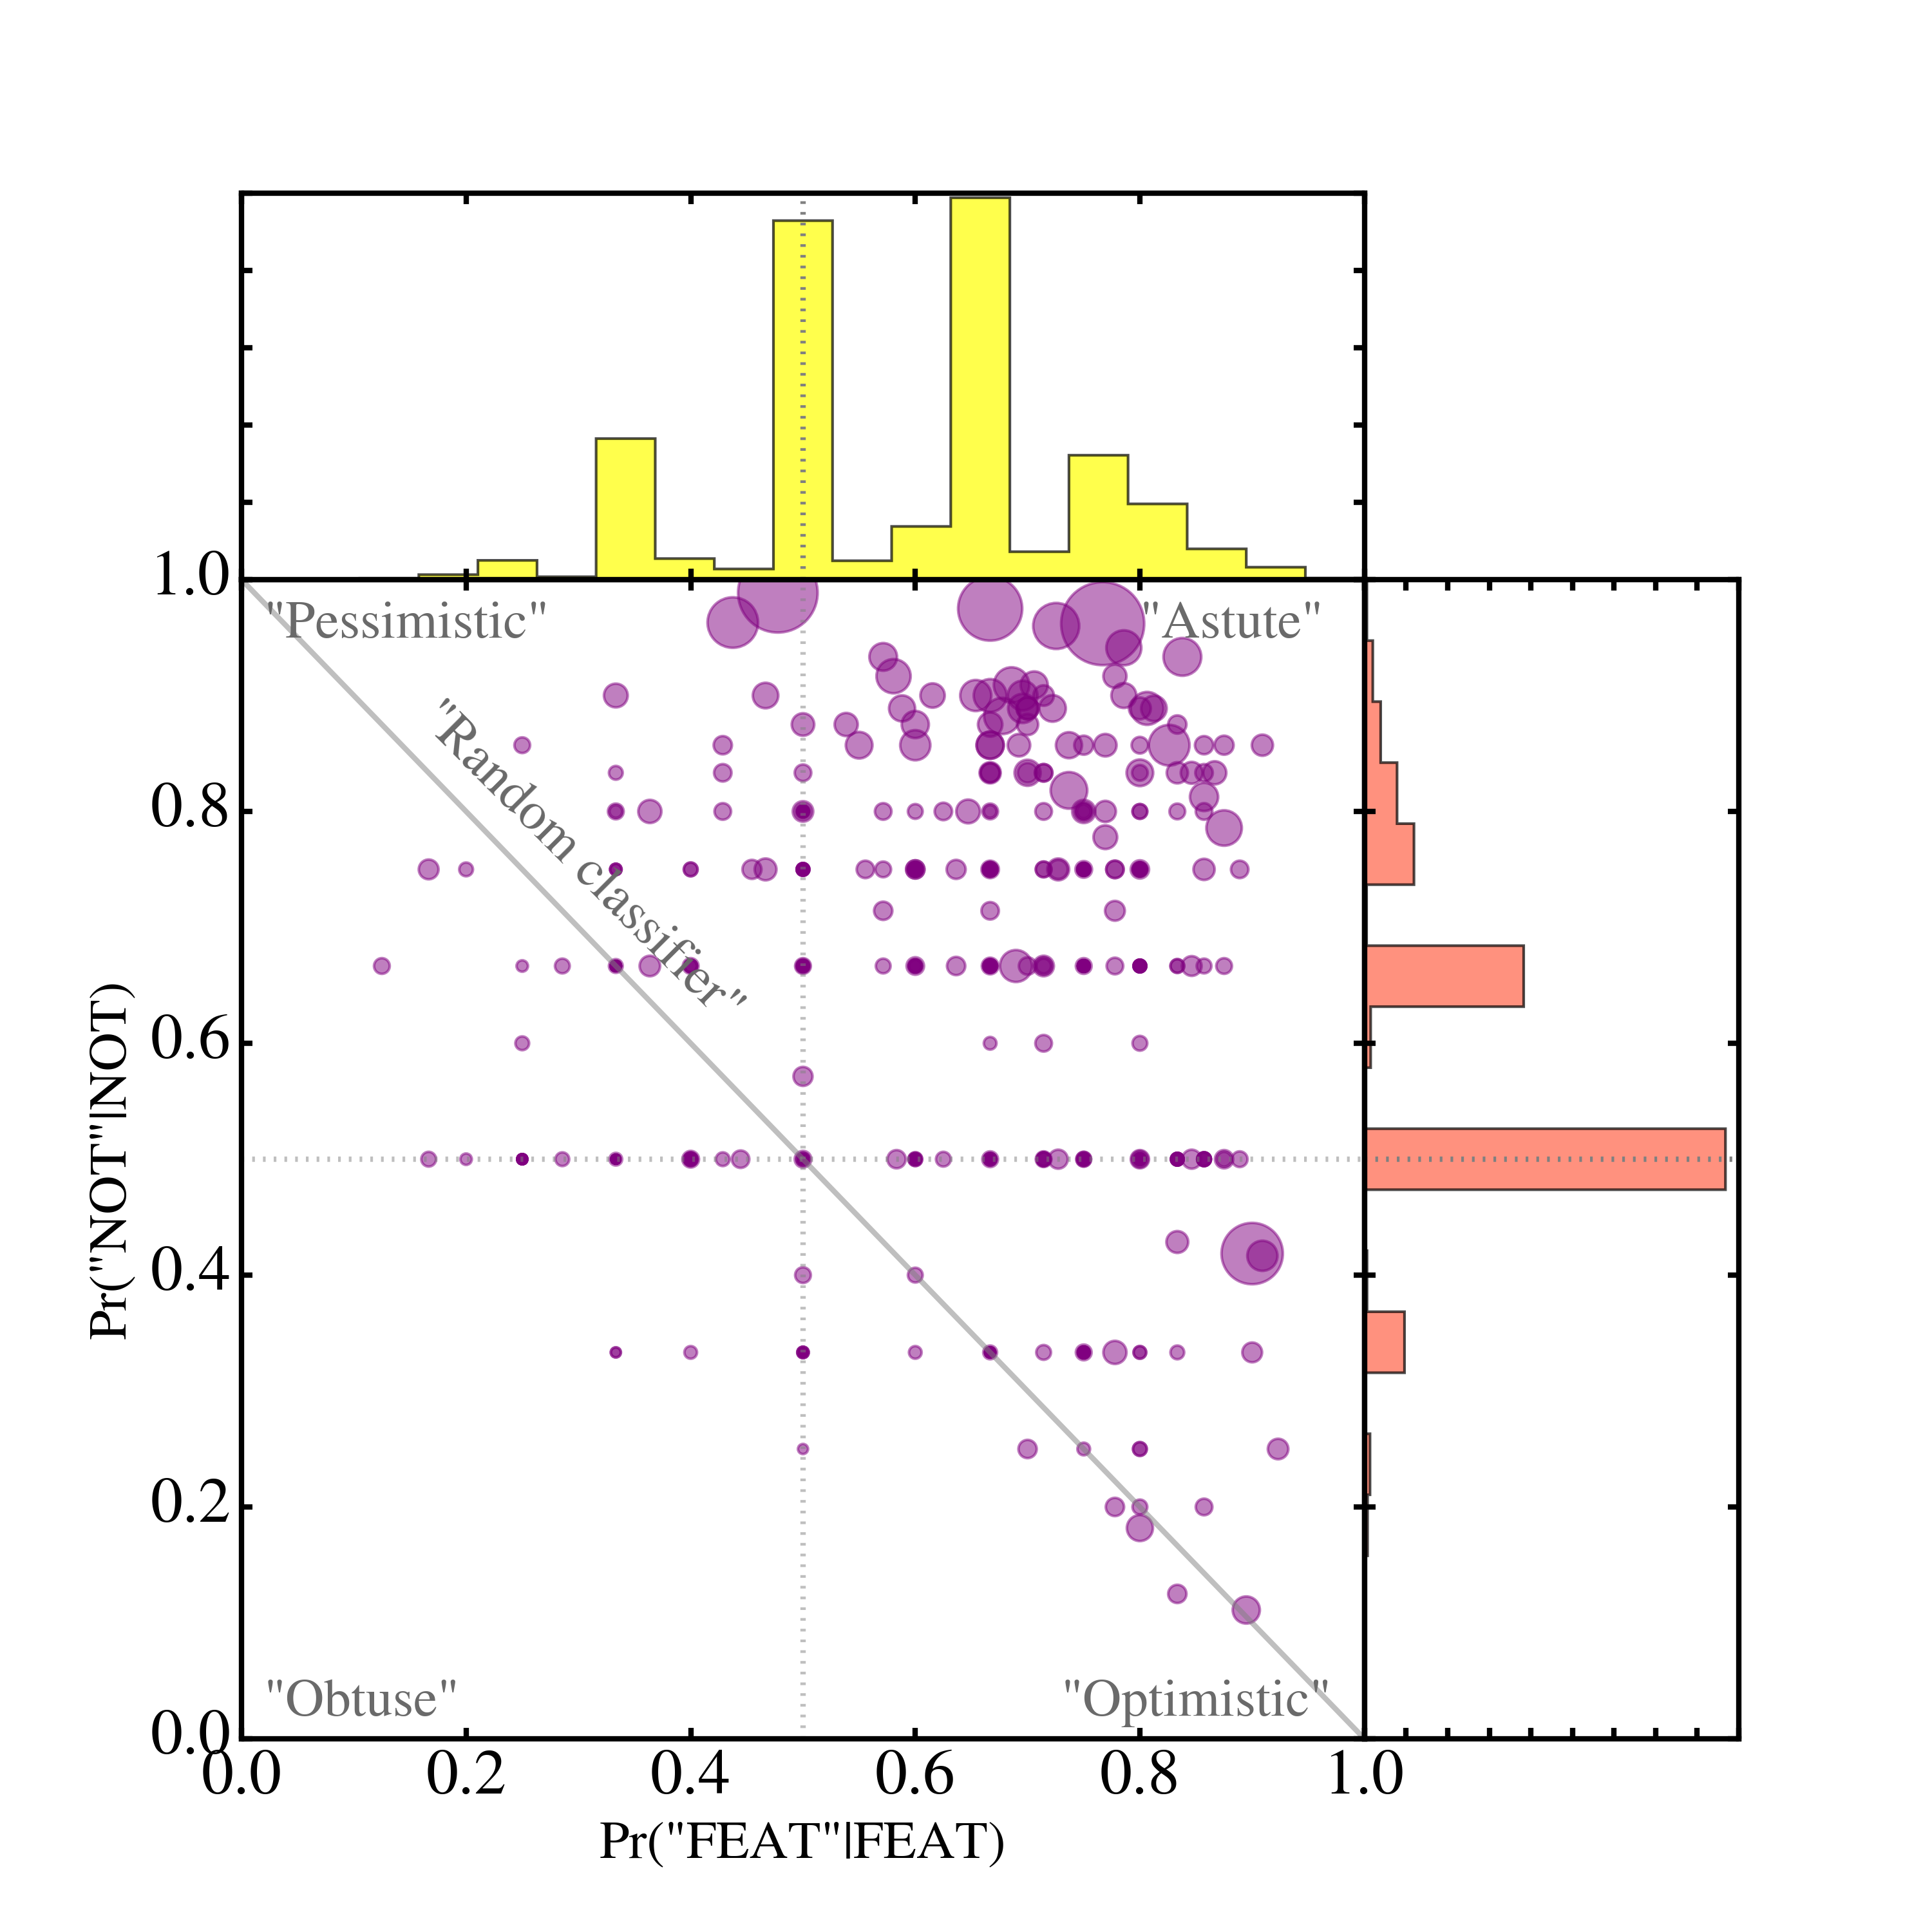
\includegraphics[width=3.7in]{figures/test_user_probs.png}
\caption{Confusion matrices for 1000 GZ2 volunteers where the size of the circle is proportional to the number of training images that volunteer classified. The distributions on the right and top represent the full sample of $\sim$30K volunteers. A quarter of GZ2 volunteers are ``Astute" meaning that they are adept at correctly identifying both~\feat~and~\notfeat~subjects. The peaks at 0.5 in both distributions are an artifact of training: a majority of volunteers see only one training image which updates only one half of their confusion matrix. \label{fig: volunteer training}}
\end{figure}

%We find that the SWAP algorithm does not perform well without the use of designated training images. Furthermore, SWAP performs optimally when these training images re introduced towards the beginning of a volunteer's contribution to the project. This allows each volunteer's confusion matrix to update sufficiently before intense classification of test images commences. 

We select a sample of $\sim$3500 SDSS galaxies for which we obtain expert classifications through the Zooniverse platform.\footnote{The Project Builder template facility can be found at \url{http://www.zooniverse.org/labs.}}
%which overlaps the \cite{NairAbraham2010} catalog. This catalog contains $\sim$14K galaxies classified by eye into various T-Types, a numerical index of a galaxy's stage along the Hubble sequence. Though helpful, this particular classification isn't directly comparable to GZ2 as discussed in~\cite{Willett2013}. Therefore, we took the additional step of
These classifications were provided by approximately 15 members of the
Galaxy Zoo science team. % ranging from advanced graduate students, post docs, and faculty.
 The question posed was identical to the original GZ2
question and at least five experts saw each galaxy. %Once classifications were complete,
Votes were aggregated and a simple majority was used to provide an expert label to
each of the 3500 subjects. 
%Not  every volunteer in the GZ2 database classified at least one of these ad hoc training images. Because we wish to recreate the conditions of the Space Warps project, 
Our final dataset consists of the classifications made 
by those volunteers who classify at least one of these expertly-identified galaxies. 
We thus retain $\sim$14 million classifications from $\sim$30K unique volunteers. 
%This reduces our raw data set from
%16 million classifications to 14 million; from 90K unique volunteers to 30K. 
Training image classifications are processed first in all of our simulations. 

%Finally, the classifications for these particular subjects could have timestamps anywhere within the 14-month time span during which the original project ran. We therefore adjust the order of the classification timestamps such that annotations of training sample subjects have timestamps well before all other GZ2 subjects. 
%Since it is implicitly assumed that a subject's classifications are independent and random, the order of the classifications should have a small effect, if any, on the results.   which pulls from the database according to timestamps,

%the training image classifications are the first to be processed with SWAP. 
%In all of our simulated runs, the first four days consist of processing training 
%image classifications after which the remaining GZ2 subjects classifications are processed.


%%%-------------------------------------------------------
%%%  FIGURE:    SWAP FIDUCIAL RUN
%%%-------------------------------------------------------
\begin{figure*}[ht!]
\plotone{figures/GZX_eval_and_retirement_baseline_4paper.png}
\caption{Fiducial SWAP simulation demonstrating the dramatic increase in the subject retirement rate as a function of GZ2 project time (in light blue) compared with the original GZ2 project (dark blue) corresponding to the left axis. Not only is efficiency increased by a factor of four or more, we maintain high quality classifications as shown by high marks in accuracy, completeness and purity which correspond to the right axis.  Specifically, these metrics are computed on the sample obtained by that day in GZ2 project time, e.g. on day 20, these metrics are computed on the 120K subjects which SWAP has classified by that time; their SWAP labels compared to `true' labels derived from published GZ2 data. \label{fig: fiducial run}}
\end{figure*}

Figure~\ref{fig: volunteer training},
%demonstrates the volunteer training we achieve with this scheme 
adapted from~\cite{Marshall2016}, shows confusion matrices for 1000 volunteers,
where the size of the circle is proportional to the number of training images that
volunteer classified. The histograms represent the distribution of each component
of the confusion matrix for all volunteers.
 Nearly 25\% of volunteers are considered `Astute'  indicating
they are generally good at correctly identifying both~\feat~and~\notfeat~subjects.
The spikes at $0.5$ in the histograms are due to the 48\% of volunteers that see only one 
expertly-classified training image (i.e.,~\feat), leaving their probability in the 
other (\notfeat) unchanged.
Additionally, 4\% of volunteers have a confusion matrix of (0.5, 0.5) indicating these 
volunteers classified two training images of the same type, one correctly and 
one incorrectly. 


%%----------------------------------------------------------------------------------------------------------------------------------------------------
%%   Subsection:    		SWAP only (FIDUCIAL RUN)
%%----------------------------------------------------------------------------------------------------------------------------------------------------
\subsection{Fiducial SWAP simulation}\label{sec: fiducial}

To simulate a live project, we run SWAP on a time step of $\Delta t = 1$ day, during 
which SWAP processes all volunteer classifications with timestamps within that range.
This is performed for three months of GZ2 classification data. 
For our fiducial  simulation we start all confusion matrices at (0.5, 0.5), and set the initial subject prior probability, \p~$= 0.5$. We set the~\feat~threshold, \tf, i.e., the minimum probability for a subject to be retired as~\feat, to $0.99$. Similarly, we set the~\notfeat~threshold, \tn~$= 0.004$. In Appendix~\ref{sec: tweaking swap}
we explore how these initial parameters affect the SWAP output.
%However, before a simulation can be run, a number of parameters which control the behavior of SWAP must first be chosen. These include the initial confusion matrix assigned to each volunteer, the retirement thresholds, and the prior probability of the subject. Specifically, we must choose 
%\begin{itemize} 
%\item \Pf, the initial probability that a volunteer identifies a subject as being~\feat, $P_0(``F"|F)$
%\item \Pn, the initial probability that a volunteer identifies a subject as being~\notfeat, $P_0(``N"|N)$
%\item \p, the prior probability of a subject to be~\feat.
%\item \tf, the threshold defining the minimum probability for a subject to be retired as~\feat.
%\item \tn, the threshold defining the maximum probability for a subject to be retired as~\notfeat.
%\end{itemize}



Because our goal is to increase the efficiency of galaxy classification,
we use as a metric the cumulative number of retired subjects
as a function of the original GZ2 project time.
%GZ2 retirement was defined by the number of volunteer classifications.  
%requiring $\sim$40 individual volunteers to reach classification consensus for each subject. 
We define a subject as GZ2-retired once it achieves 30 volunteer votes since 
not every subject reached the 40 volunteer threshold as discussed in~\cite{Willett2013}. 
A subject is considered SWAP-retired once its posterior 
probability crosses either of the retirement thresholds defined above. 

However, it is important not to prioritize efficiency at the expense of quality. 
We thus also consider the metrics of accuracy, 
purity and completeness as a function of GZ2 project time.  These are 
defined as follows: accuracy is the number of correctly
identified subjects divided by the total number retired; completeness is the number of 
correctly identified~\feat~subjects divided by the number of actual~\feat~retired; 
and purity is the number of correctly identified~\feat~subjects divided by 
the number of subjects retired as~\feat. Thus, a complete sample has no false
negatives whereas a pure sample has no false positives. 

We compute these metrics by comparing the SWAP-assigned labels of
the cumulatively retired subject set  to the~\raw~labels for each day of
the simulation. 
%Using the~\raw~labels as truth, we compute the above metrics on the 
%subject set retired by that day of the GZ2 project.
For example, Figure~\ref{fig: fiducial run} shows that by Day 20, 
SWAP retired 120K subjects. Comparing those SWAP labels to~\raw~labels, 
we find that the sample is 96\% accurate, 99.7\% complete, and 92\% pure. 
Furthermore, the metrics computed on the final day of the simulation
reflect the quality of the full SWAP-retired sample. 
%(that is, of all the subjects we retire up to that point, we successfully identify all that are~\feat),and 92\% pure. 

Figure \ref{fig: fiducial run} shows the results of our fiducial SWAP simulation
compared to the original GZ2 project. The left axis shows the cumulative
number of retired subjects as a function of GZ2 project time. 
By the end of our simulation, GZ2 retires $\sim$50K subjects while SWAP retires 
more than 225K. 
We thus classify 80\% of the entire GZ2 sample in three months. 
As the original GZ2 project took approximately a year to complete, this
represents a factor of four increase in the rate of classification. 
%We thus achieve a factor of four increase in the rate of classification. 

We also consider the reduction in human effort required to classify
this subject set. Figure~\ref{fig: swap vote distributions} shows the 
distribution of the number of volunteer classifications per subject 
achieved through SWAP (light blue) and GZ2 (dark blue). 
As expected, GZ2's distribution peaks around $\sim$45 indicating that, on average,
45 unique volunteers classify each subject. On the other hand, SWAP's
distribution peaks around 9 classifications per subject. 
Furthermore, subjects that are `easy' to classify (i.e.,~\feat) require
even fewer classifications to reach strong consensus. 
More precisely, SWAP processed a total of $2.3 \times 10^6$ volunteer 
classifications while GZ2 required $\sim$$10^7$ for the same subject set. 
Again, this is more than a factor of four reduction in human effort. 


%Some subjects are `easy' to classify and can be retired in as few as three classifications, while subjects with less consensus will take more classifications, each one kicking the subject back and forth in probability space before it eventually crosses one of the retirement thresholds. This explains the tail towards larger classification number.

%%%-------------------------------------------------------
%%%  FIGURE:   SWAP vote distributions
%%%-------------------------------------------------------
\begin{figure}[t!]
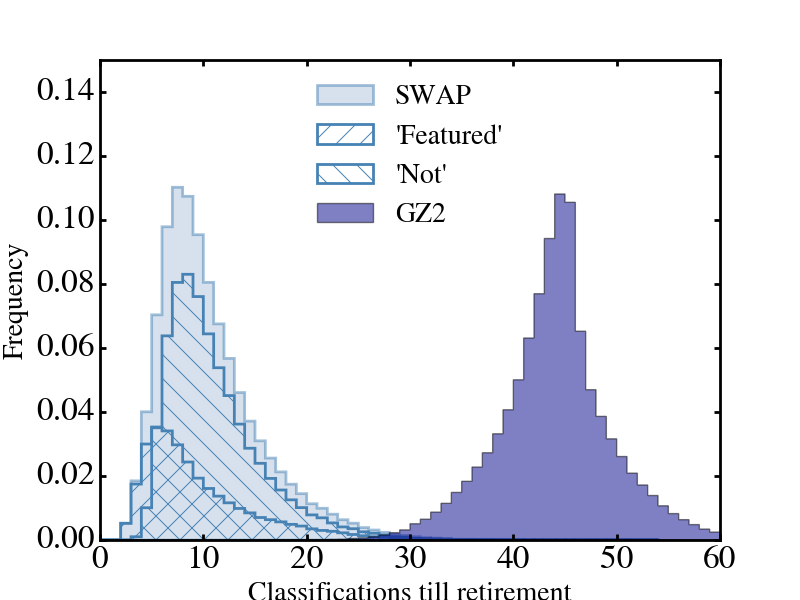
\includegraphics[width=3.65in]{figures/GZX_clicks_till_retired_baseline.png}
\caption{SWAP requires four times less human effort than GZ2 as evidenced by the distribution of the number of classifications a subject receives before retirement for the $\sim$225K subjects retired during our fiducial run.  As expected, the GZ2 distribution peaks around 45 classifications per subject. In contrast, most subjects need only 10 classifications when processing volunteer votes with SWAP.  \label{fig: swap vote distributions}}
\end{figure}

%We have shown that by clever and adaptive processing of volunteer classifications, efficiency of subject retirement can be increased by a factor of four. The rate and quality of subject retirement will be, in part, a function of initial SWAP parameters. We explore in depth the SWAP parameter space in Appendix~\ref{sec: tweaking swap}.
%We now turn to a discussion of how classification and retirement change as a function of SWAP input parameters. 


\subsection{Disagreements between SWAP and GZ2}

%%%-------------------------------------------------------
%%%  FIGURE:   SWAP failures
%%%-------------------------------------------------------
\begin{figure}[t!]
\includegraphics[width=3.2in]{figures/swapgetsitwrong_cropped.png}
\caption{The right panel shows the distribution of GZ2 `features or disk' + `star or artifact'  raw vote fractions for subjects identified as false positives (blue) and false negatives (red). The solid distribution represents all subjects retired by SWAP. Vote fractions between 0.4 and 0.6 indicate that volunteers were uncertain on the nature of those subjects.  That SWAP doesn't assign a matching label is not surprising.  \label{fig: SWAP sucks}}
\end{figure}
%Furthermore, it is unsurprising that these same subjects are physically more difficult to classify being, on average, smaller and fainter than the sample as a whole as shown in the right panel. 

Galaxy Zoo's strength comes from the consensus of dozens of volunteers voting on each subject. 
Processing votes with SWAP reduces the number of classifications to reach consensus. 
Though we typically recover the~\raw~label, SWAP disagrees about 5\% of the time. 
We thus examine the false positives (subjects SWAP labels as~\feat~but~\raw~labels as~\notfeat) and false negatives (subjects SWAP labels as~\notfeat~but~\raw~labels as~\feat).


%In this section we examine the effects driving this disagreement. 
%whereby we again  turn to our fiducial simulation, 
We find that the majority of these disagreements are due to uncertainties in 
the~\raw~label. Figure~\ref{fig: SWAP sucks} shows the distribution of the GZ2 
raw vote fraction for all subjects retired by SWAP (solid black line), the 
false positives (blue), and the false negatives (red).  Here, $f_{features}$ is 
the fraction of volunteers who classified a subject as~\feat, and equivalently for
$f_{artifact}$. A combined fraction greater than 0.5 defines a~\feat~galaxy
according to our~\raw~labels. The majority of incorrectly 
labeled subjects have $0.4 \le f_{features}+f_{artifact} \le 0.6$, indicating that 
the GZ2 raw vote fractions are simply too uncertain to provide high quality labels. 

%Recall that we group these together as~\feat~during  our SWAP simulations and so group them here for a fair comparison. Furthermore, because we used a majority vote fraction to derive labels, any subject with $ f_{features}+f_{artifact} > 0.5$ would be labeled~\feat.  However the false negative (red) distribution shows that a portion of these still attained a~\notfeat~label through SWAP (with the opposite being true for the blue false positive sample). In fact, 

Two smaller effects contribute to the disagreement between SWAP and GZ2. 
First, as the number of classifications used to retire a galaxy decreases, the 
likelihood of misclassification by random chance increases. 
Second, disagreement arises due to expert-level volunteers whose confusion 
matrices are close to 1.0. These volunteers are essentially more 
strongly weighted allowing that subject's posterior to cross a retirement threshold
in as few as two classifications. In some cases, these expert-level volunteers disagreed 
with the majority. These issues can be mitigated by requiring each subject reach 
a minimum number of classifications before allowing its probability to cross a 
threshold thus combining the best qualities of GZ2 and SWAP. 

%Volunteers generally do not have (\Pf,~\Pn) = (0.5, 0.5). We find that, occasionally, some subjects are retired with only two classifications.  This can occur when a volunteer achieves exceptionally high probabilities in their confusion matrix. While these volunteers may have attained `expert' status and ultimately provide a correct response, they do not always agree with the~\raw~labels. We estimate this effect at XXX. 

%Another effect contributing to the disagreement is related but more subtle and concerns the order in which volunteers cast their votes. Consider a subject where the first N volunteers classify it as X while the subsequent majority of volunteers classify the subject as Y. Here the power of GZ2's large consensus shines because this lopsided voting is averaged out. SWAP, however, will swiftly kick that subject's probability over a retirement threshold when encountering such a chain of classifications. The result is SWAP labels which disagree with GZ2 labels purely due to order statistics. Consider a subject with a $f_{features}+f_{artifact} = 0.2$, where 40 unique volunteers have classified this subject yielding a GZ2 label of~\notfeat. What is the probability that this subject will obtain a label~\feat~through SWAP? In other words, what is the probability that the first eight volunteers all voted~\feat?  If we assume all volunteers have~\Pf~= 0.5, it is trivial to compute $1/2^8 = 0.39\%$. Of course, this effect is more complicated to model in aggregate since volunteers have confusion matrices that vary with time and subjects can be retired with a varying amount of volunteer classifications. 

%This leads to another subtle effect that can cause SWAP labels to disagree with GZ2 labels.

%To mitigate these issues one could a.) require each volunteer classify a certain number of subjects to increase their confusion matrix values or b.)  The difference lies between averaging over a volunteer's burn-in phase versus a subject's burn-in phase. The latter is preferable as the majority of Zooniverse volunteers contribute only a small number of classifications to any given project. Requiring they achieve a minimum classification count before allowing their contribution to count would hamstring the effectiveness of citizen science projects. 


\subsection{Summary}

We demonstrate a factor of four or more increase in 
classification efficiency while maintaining accuracy over 95\%, nearly perfect 
completeness of~\feat~subjects, and with a purity that can be controlled by careful 
selection of input parameters to be better than 90\% (see Appendix~\ref{sec: tweaking swap}).
We explore those subjects wherein SWAP and GZ2 disagree and conclude that 
the majority of this disagreement stems from uncertainty in~\raw~labels.
We now turn our focus towards incorporating a machine
classifier utilizing these SWAP-retired subjects as a training sample. 


%%----------------------------------------------------------------------------------------------------------------------------------------------------
%%   INTEGRATING MACHINE CLASSIFIERS 
%%----------------------------------------------------------------------------------------------------------------------------------------------------
\section{Efficiency through incorporation of machine classifiers} \label{sec: machine}

In this section we construct the full Galaxy Zoo Express by incorporating supervised 
learning, the machine learning task of inference from labeled training data. 
The training data consist of a set of training examples, and must include
an input feature vector and a desired output label.  Generally speaking,
a supervised learning algorithm analyzes the training data and produces an inferred 
function that can then be mapped to new examples. An optimized algorithm will 
correctly determine class labels for unseen data. In general, most classification 
algorithms can handle prediction of several labels simultaneously. Work has been
done to predict the entirety of GZ2 classification labels using deep learning 
\citep{Dieleman2015} with great success. 
However, it is still simpler for a machine to predict fewer labels than it is to predict several dozen, \textbf{[citation?]}, 
with the additional bonus that fewer class labels require less training data. 
By processing human classifications through SWAP we obtain a discrete, binary task
for a machine to tackle. We briefly outline the technical details of our machine
classifier before turning towards the decision engine we develop for GZX in 
section~\ref{sec: decision engine}. 


\subsection{Random Forests}
Because our task is simple, we choose a simple machine. In particular, we use 
a Random Forest (RF) algorithm,  an ensemble classifier that operates by bootstrapping
the training data and constructing a multitude of individual decision tree algorithms, 
one for each subsample.  An individual decision tree works by deciding which of 
the input features best separates the classes. It does this by performing 
splits on the values of the input feature that minimize the classification 
error. These feature splits proceed recursively. As such, decision trees alone are
 prone to overfitting the training data thus precluding them from generalizing 
well to new data. Random Forests mitigate this effect by combining the 
output label from a multitude of decision trees.  In particular we use the 
\texttt{RandomForestClassifier} from the Python module \texttt{scikit-learn}
\citep{scikit-learn}. 

\begin{comment}
%One of the simplest algorithms to conceptualize and use is the K-nearest neighbors (KNN) classifier. This classifier works simply by considering the K neighbors nearest to the test point in Euclidean space. As we have only a binary classification challenge, the test point is classified according to the majority of its K neighbors. In the event of a tie, the label if the closest neighbor to the test point determines its class. Though simplistic, this algorithm is surprisingly powerful in that it performs well in higher-dimensional space and is relatively fast to train. Obviously, the most important parameter to consider is the number of nearest neighbors to assign to each test point. But this is pretty much the only knob to turn in this method which is another benefit -- ease of interpretation. 
%We use scikit-learn's implementation of K-Nearest Neighbor Classifier (KNC) and optimize the K parameter. 
\end{comment}


\subsection{Cross-validation}
Of fundamental importance is the task of choosing an algorithm's hyperparameters, 
values which determine how the machine learns.  In the case of a RF, these include
 the maximum depth of the tree, the minimum leaf size, the maximum
number of leaf nodes, etc. The goal is to determine which values will optimize 
the machine's performance and thus cannot be chosen \textit{a priori}. 
We perform a $k$-fold cross-validation whereby the 
training sample is split into $k$ subsamples. One subsample is withheld to 
estimate the machine's performance while the remaining data is used to train the machine. 
This is performed $k$ times and the average performance
value is recorded. The entire process is repeated for every combination of the 
 hyperparameter space and values that optimize the output are chosen. 

%Ideally, one would train the machine with every combination of parameters and consider the resulting performance by testing the trained machine on a sample withheld from the training sample so as not to contaminate the results. Formally, 
 
\subsection{Feature Representation and Pre-Processing}
Machine learning algorithms require a feature vector for each training example. 
This vector is composed of D individual numeric quantities associated with the 
subject which the machine will use to discern that subject from others in the 
training sample. To segregate~\feat~from~\notfeat, we draw
on ZEST \citep{Scarlata2007} and compute concentration, $C$, asymmetry, $A$, 
Gini coefficient, $G$, and M$_{20}$. Coupled with SExtractor's measurement 
of ellipticity \citep{sextractor}, we provide the machine with a five dimensional morphology parameter space. 
(See Appendix \ref{sec: measuring morphology} for details of the measurement process.)
These non-parametric diagnostics have long been used to 
quantify galaxy morphology in an automated fashion \cite[e.g.,][]{Abraham1996, Bershady2000, Conselice2000, Abraham2003, Conselice2003, Lotz2004, Snyder2015}.
%Altogether, these features describe a five dimensional parameter space in which the machine attempts to distinguish between the two classes. As the RF algorithm is capable of handling high-dimensional parameter spaces, in a future paper we will explore increasing our feature space to include parametric morphology indicators such as Sersic index and B/T ratio. 

One particular benefit of the RF algorithm is the flexibility with which it can accept input 
features. Most algorithms require that each feature dimension lie on the same scale. 
This is not necessary with a RF. The only preprocessing required is the removal of morphological parameters which were not well measured, i.e. catastrophic failures. 

%\textbf{Should this paragraph be here? Probably not. But it should be somewhere?}
%This is quite distinct from \textit{deep learning} methods which can learn on every 
%pixel of an image through a series of non-linear transformations. This technique has
%been successful at predicting galaxy morphology labels as explored by 
%\cite{Huertas-Company2015}, \cite{Dieleman2015} and others. In this work our focus
%is to outline a practical method to efficiently combine human and machine classification,
%not seek the most optimal or accurate machine algorithm. We are concerned more 
%with speed and simplicity though we stress that a machine is just an algorithm. 
%In the future, this particular application will accommodate any algorithm, including 
%deep learning techniques, should they so be desired. 

%Though deep learning methods promise new heights of classification accuracy, there are some drawbacks. Most notably, the interpration of these methods in the context of physical quantities is lacking. Because of the complex suite of layered non-linear transformations, it is difficult to backstrapolate what qualities of the image were most successful at understanding that galaxy's morphology. Moreover, connecting that to physical mechanisms within the galaxy remains to be seen. On the other hand, much work has been invested in connecting aggregate features such as CAS, G-M20 which are well demonstrated to correlate with specific galaxy stuffs like SFH and ... whatnots.. and described below.


%Before we feed the algorithm with these feature vectors we first perform two pre-processing steps. First, we clean the data as there are some very few number of cases where our algorithm failed to recover appropriate values for the Petrosian radius, C, A, G, or M20. Our code represents these failures as infs or nans and we thus remove these subjects from all samples.  The second transformation puts each of the features on equal footing. Taken at face value, each of the five morphology parameters resides in a different range of values:  M20 is nearly always negative as it is logarithmic, while Asymmetry and Gini are always between 0 and 1.  In order for the machine classifier to treat all features equally we scale each feature along columns. If a row represents an individual subject, then a column represents the same feature for all subjects. We normalize each subject's features in the standard way: 
\begin{comment}
\begin{equation}
z_{feature} = \frac{f_i - \mu}{\sigma}
\end{equation} 
Where $f_i$ is the $i$th subject's feature value, $\mu$ is the mean of the entire feature sample, and $\sigma$ is the standard deviation of the entire feature sample. This scales each feature to values between 0 and 1. 
\end{comment}



%%%-------------------------------------------------------
%%%  FIGURE:   LEARNING CURVE
%%%-------------------------------------------------------
\begin{figure}[t!]
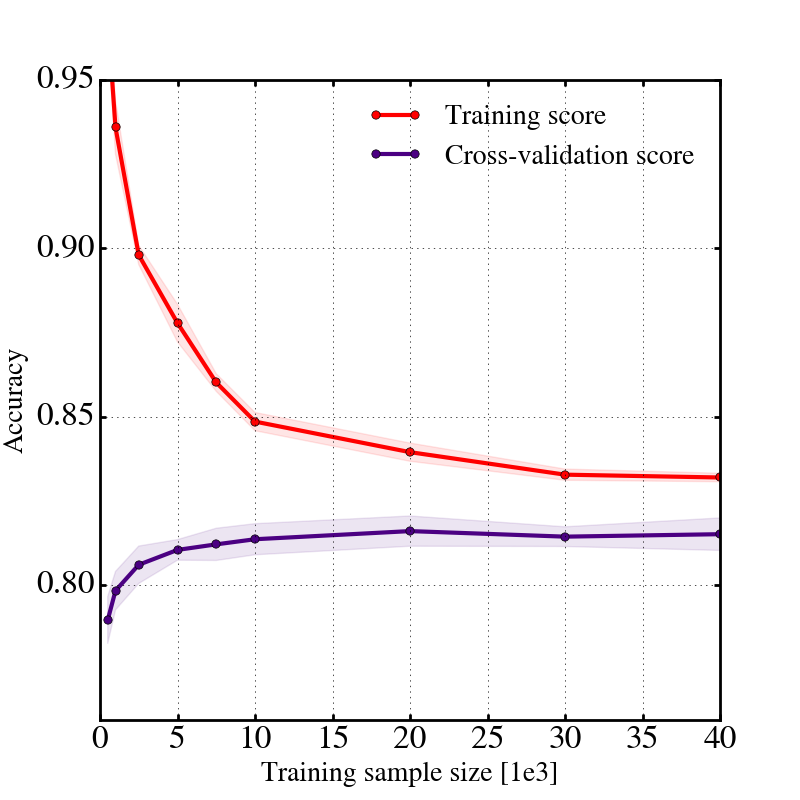
\includegraphics[width=3.25in]{figures/learning_curve_RF.png}
\caption{Learning curve for a Random Forest with fixed hyperparameters (maximum depth of tree, number of trees, etc.). The training score is the accuracy of the trained machine applied to its own training sample. The cross-validation score is the accuracy of the machine computed during the cross-validation process. When the training sample size is small, the machine is able to accurately identify its own training sample but is unable to generalize to unseen data, as evidenced by a low cross-validation score. As the training sample size increases, the cross-validation score increases demonstrating that the machine is more adept at generalization. This behavior plateaus indicating that larger training sample sizes provide little in additional performance. \label{fig: learning curve}}
\end{figure}
%\subsection{Training and Validation Samples}
%The training sample again for the machine is dynamically generated through SWAP-retired
%subjects as discussed in detail in section~\ref{sec: SWAP}. 
%As we showed in the previous section, SWAP retires subjects far more rapidly than GZ2 by adaptively tracking volunteer skill and subject probabilities in a Bayesian framework. This provides us with a way of quickly generating large subject samples with accurate labels provided by human classifications that are dynamically generated as a function of GZ2 project time. 
%For the following analysis we build off of our fiducial model where, according to Figure~\ref{fig: fiducial run}, SWAP retires XXX subjects within 10 days. 

%In addition to a training sample we also desire a validation sample to estimate the generalization (true) error of our trained machine. We  utilize our expert-classified sample again for this purpose. 
%For this purpose we maximize the utility of our expertly classified sample. This sample thus provides training to our volunteers and verification for our machine. 

\subsection{Decision Engine}\label{sec: decision engine}
A number of decisions must be made before attempting to train the machine. 
Which subjects should be designated as the training sample? 
When should we attempt the first training session? 
How do we decide when the machine has successfully trained enough to be
applied to unseen subjects? These are the core issues that we address
in our machine learning decision engine.

\textbf{Which subjects should provide the training sample?} 
As discussed in detail in~\ref{sec: SWAP}, SWAP
yields a probability that a subject exhibits the feature of interest. A RF requires
distinct classes so we use only those subjects which have crossed either of the 
retirement thresholds. However, subjects do not cross these thresholds with equal rates. 
At any given stage in the simulation, the ratio of retired~\feat~to~\notfeat~is not
guaranteed to be balanced which lead to sub-optimal learning.
 However, as a first test, we allow the machine to train on all high probability subjects. 

\textbf{When should we attempt the first training session?}
SWAP retires a few hundred subjects in the first days of the simulation.
One could, in principle, train a machine with such a small sample, but the resulting
predictions on the test sample will be exceptionally poor. Furthermore, the machine
won't know that it's performing poorly. 
%For example, if a training sample consists of 100~\feat~subjects, the machine will subsequently predict that every member of the test sample is also~\feat~with high probability. This is obviously wrong. 
In practice, a much larger training size is required for the machine to learn the 
true parameter space. There is no hard rule for choosing this number, but a RF 
is a simple model so we initially require at least 10K subjects before attempting the first training session. 


\textbf{When has the machine trained enough?} 
We assess the machine's training by considering a learning curve, 
an illustration of a model's performance with increasing sample size for fixed 
model hyperparameters. An example is shown in Figure~\ref{fig: learning curve}.
 The cross-validation score is the accuracy resulting from k-fold cross-validation. 
The training score is the resulting machine applied to the training sample. 
When the sample size is small, the cross-validation score is low while the training score is high. 
This is a clear demonstration of a model over-fitting the data. 
As the training sample size increases, the cross-validation score increases and 
eventually plateaus signifying that 
%Eventually both plateau, regardless of how large the training sample grows.  This demonstrates that, after a certain point, for a fixed complexity model, 
larger training sets will  yield little additional gain. 
%That the training score reduces almost to the cross-validation score signifies that this particular model is not well suited to capturing the complexity of the data set. A more sophisticated model would, in turn, likely require a larger training sample. 

We use this general feature of any machine learning process to guide our 
decision making by looking for the characteristic 
%We cannot reproduce a true learning curve because the cross-validation procedure we perform can, in principle and in practice, yield a different set of machine hyperparameters that are most appropriate for the training sample it received that night.  Instead, we look for the characteristic 
cross-validation score plateau. At each timestep, we record
the machine's training performance, including how well it scores on the 
training sample (to estimate overfitting), cross-validation score, 
and the best hyperparameters. When the machine's 
cross-validations score remains within 1\% on three consecutive nights, 
we deem the machine's performance acceptable. 


\subsection{The Machine Shop}\label{sec: machine shop}
We can now describe a full GZX simulation. A typical run begins with human classifications 
processed through SWAP for several days. During that time, humans `train' on the 
gold standard sample and then begin classifying the main sample.  Once they retire 
at least 10K subjects, these are passed to the machine which trains for the first time. 
A suite of performance metrics are recorded by a machine agent, similar
in construction to SWAP's agents. Each night, the machine agent determines 
whether or not the machine has sufficiently trained by assessing all previous nights of 
training, comparing the variation in performance metrics. Once the machine has
passed the criterion laid out above, the agent introduces the machine to the test sample
which consists of any subject that has not yet been seen by humans, has not yet 
reached retirement through SWAP, has not been previously classified by itself, 
and is not part of the gold standard sample.  

What constitutes a machine classification? Once the trained machine is applied to
the test sample it will provide predictions for every subject therein, but these predictions
are not made with the same certainty. Most machine algorithms allow one to obtain
a probability associated with each subject's predicted label. 
In the case of an RF, this probability is simply the average of the probabilities of each 
individual decision tree where the probability of a single tree is determined as the fraction
of subjects of class X on a leaf node.  We use this probability to assess subjects about which
the machine is most confident (though we note it is not a true measure of confidence).
Only subjects that receive a class prediction with $p_{machine} \ge 0.9$ are considered
retired and hence removed from the system. The remaining subjects have the possibility 
of being classified by humans (or the machine again) during future timesteps. 


%This is the embodiment of our feedback loop. Those subjects on which the machine is least confident can be examined by human classifiers, potentially becoming part of the training sample during a future cycle. Ideally, this increased training sample will cover a larger portion of the parameter space in which the machine can learn. With additional subjects spanning all of the parameter space, the machine can quickly achieve its maximum performance. 

%In the future we will create a more sophisticated feedback mechanism whereby we can send particularly challenging subjects to expert-level users for identification (where these users can be identified by their high confusion matrix values as determined by SWAP,  see section~\ref{sec: SWAP}). Additionally we can perform periodic spot-checks to confirm the machine's performance by cross-checking with humans for label consistency. 


\begin{comment}
In figure \ref{fig:testmetrics},
we can see how the machine is performing on the test sample as a function of 
project time. Understandably, the performance is poor the first time the machine 
crosses the `learnned` criterion. Flukes can happen and it was most likely not
quite as learned as expected or desired. However, as the project progresses the 
performance on the test sample increases. In particular, the black line denotes 
the performance as obtained on the entire test sample and we can see that even 
when the machine is at its peak, the accuracy doesn't increase much beyond 70\%. 
The red line, however, is when we select only those subjects which the machine is
most confident about (more than 90\% confidence, in particular). Now the accuracy
of the machine on this subsample reaches nearly 85\%.  

This allows us to set a criterion for which subjects the machine should be allowed
to retire from the system. We don't necessarily trust it on all subjects but can we 
trust it when it's most confident? Explore this more? 

Our system has now incorporated both clever use of human classifications and 
integrated machine classification. We now simulate the final element which is the
feedback mechanism. Those subjects which the machine is most confident about are 
flagged as retired and votes on these subjects are no longer recorded in SWAP or 
elseware. Those which the machine is not confident, however, remain in the pool 
such that, during the next timestep, volunteers can contribute to the classification 
of that subject. This will increase the diversity of the training sample thus 
providing the machine with a larger sample space in which to learn. 
\end{comment}

\begin{table*}[]
	\centering
	\caption{Summary of key quantities for GZ2 and our various simulations. All quality metrics are calculated using~\raw~labels.}
	\label{tab: summary}
	\let\mc\multicolumn
	\begin{tabular}{lcccccc}
		
		\mc7c{ \textbf{Simulation Summary} } \\
		\hline \hline
			& Days	& Subjects Retired & Human Effort 	&  Accuracy 	& Purity 	& Completeness\\
		\mc2c{} 		& 	 	& (classifications) 	&  (\%)	    	& (\%)	& (\%)	\\
		\hline
			
		Galaxy Zoo 2	&	430 	& 285962  	& 16.3 M 	& --   	& --    	 & --   \\
		SWAP only	&	92    	& 226124          & 2.3 M 	& 95.7 	& 86.7	 & 99.0     \\
		SWAP+RF      	& 32  	& 210543 	& ??? 	& 93.5    	& 84.2    	& 94.3      \\
		\hline
	\end{tabular}
\end{table*}

%%----------------------------------------------------------------------------------------------------------------------------------------------------
%%   RESULTS 
%%----------------------------------------------------------------------------------------------------------------------------------------------------
\section{Results} \label{sec: results}

%%%-------------------------------------------------------
%%%  FIGURE:    FULL GZX PERFORMANCE
%%%-------------------------------------------------------
\begin{figure}[t!]
\raggedleft
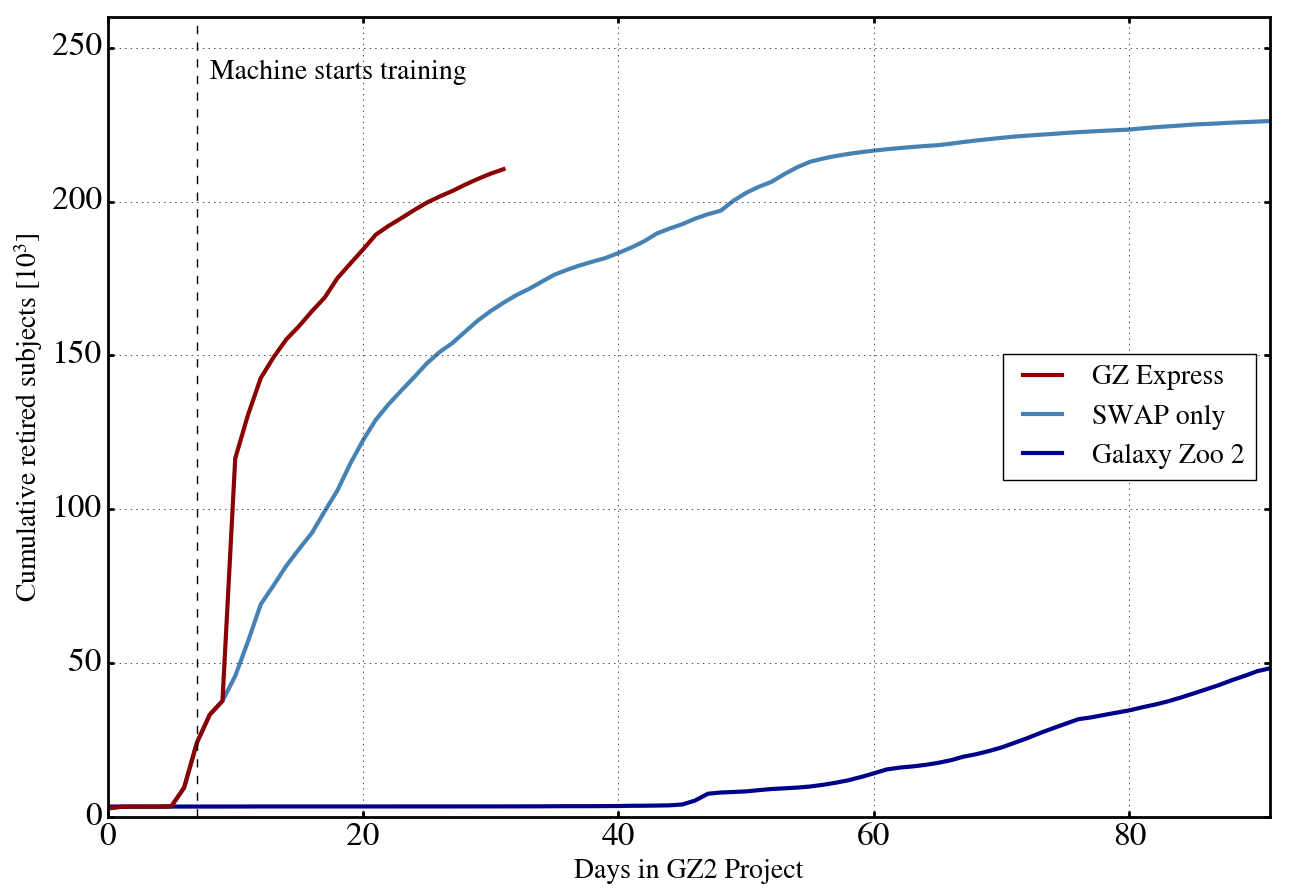
\includegraphics[width=3.45in]{figures/GZ2_sup_PLPD5_p5_flipfeature2b_RF_accuracy_redo_raw_combo_moneyplot.png}
\caption{Incorporating the machine reduces the total time to classify over 200K subjects in the GZ2 sample to just 23 days. The dashed line marks when the machine trains for the first time.  The machine trains for several nights before it is allowed to retire subjects. Both humans and machine then contribute to subject retirement. \label{fig: money}}
\end{figure}

We perform a full GZX simulation incorporating both SWAP and our RF machine using the
 fiducial SWAP run discussed in section~\ref{sec: fiducial}. 
The machine attempts its first training on Day 8 with an initial training
sample of nearly 20K subjects.  The machine undergoes several additional nights of training, 
each time with a larger training sample. 
By Day 12, the machine's agent has assessed that the machine is suitably trained. 
By this point, SWAP has provided over 40K subjects as a training sample. 
The machine predicts class labels for the remaining 230K GZ2 subjects which are not 
already retired by SWAP or part of the expertly classified sample. 
Of those, the machine strongly predicts labels ($p_{machine} >= 0.9$ for nearly 71K subjects,  immediately and dramatically increasing the overall sample of retired subjects. 
As the simulation progresses, retirement by both SWAP and
the machine tapers off, though at different rates. 
We end the simulation after 32 days, having sufficiently classified well over 200K subjects. 
We present these results in the bottom panel of Figure~\ref{fig: money} where GZX (red) 
is compared to our fiducial SWAP-only run (light blue) and GZ2 subject retirement (dark blue). 


The top panel of Figure~\ref{fig: money} shows our usual quality metrics for both 
SWAP-only and GZX, again using the~\raw~labels discussed in section~\ref{sec: data}.
Accuracy and completeness of the cumulative sample for the combined system 
each remain around 95\% and purity remains around 85\%. We note that 
incorporating the machine yields similar purity as when we 
allow SWAP to handle the entirety of the sample for a similar-sized subject set. 
Instead we seem to make a small sacrifice in the completeness of the~\feat~sample
which, in turn, affects our accuracy. Whereas SWAP alone identifies nearly all~\feat~
subjects it encounters,  the machine appears to miss a significant 
portion of these thus dropping the completeness of that day's 
cumulative sample. We discuss this behavior below.

By dynamically generating a training sample
through a more sophisticated analysis of human classifications coupled with a 
machine classifier trained through a simple feedback mechanism, we are able to 
retire over 200K GZ2 subjects in 27 days.  SWAP alone retires as many subjects in 50 days
while GZ2 requires XX months to retire as many and 14 months to retire 
the entire catalog of 285K subjects. 
GZX thus provides a full order of magnitude decrease in classification time
over the traditional crowd-sourced approach. 
We next explore the composition of those classifications.



%\multicolumn{1}{c}{}              & Days & Subjects Retired & \begin{tabular}[c]{@{}c@{}}Human Effort\\ (classifications)\end{tabular} & \begin{tabular}[c]{@{}c@{}}Accuracy\\ (\%)\end{tabular} & \begin{tabular}[c]{@{}c@{}}Purity\\ (\%)\end{tabular} & \begin{tabular}[c]{@{}c@{}}Completeness\\ (\%)\end{tabular} \\ \hline

\subsection{Who retires what, when?}  

%%%-------------------------------------------------------
%%%  FIGURE:    GZX COMPONENT CONTRIBUTIONS
%%%-------------------------------------------------------
\begin{figure}[t!]
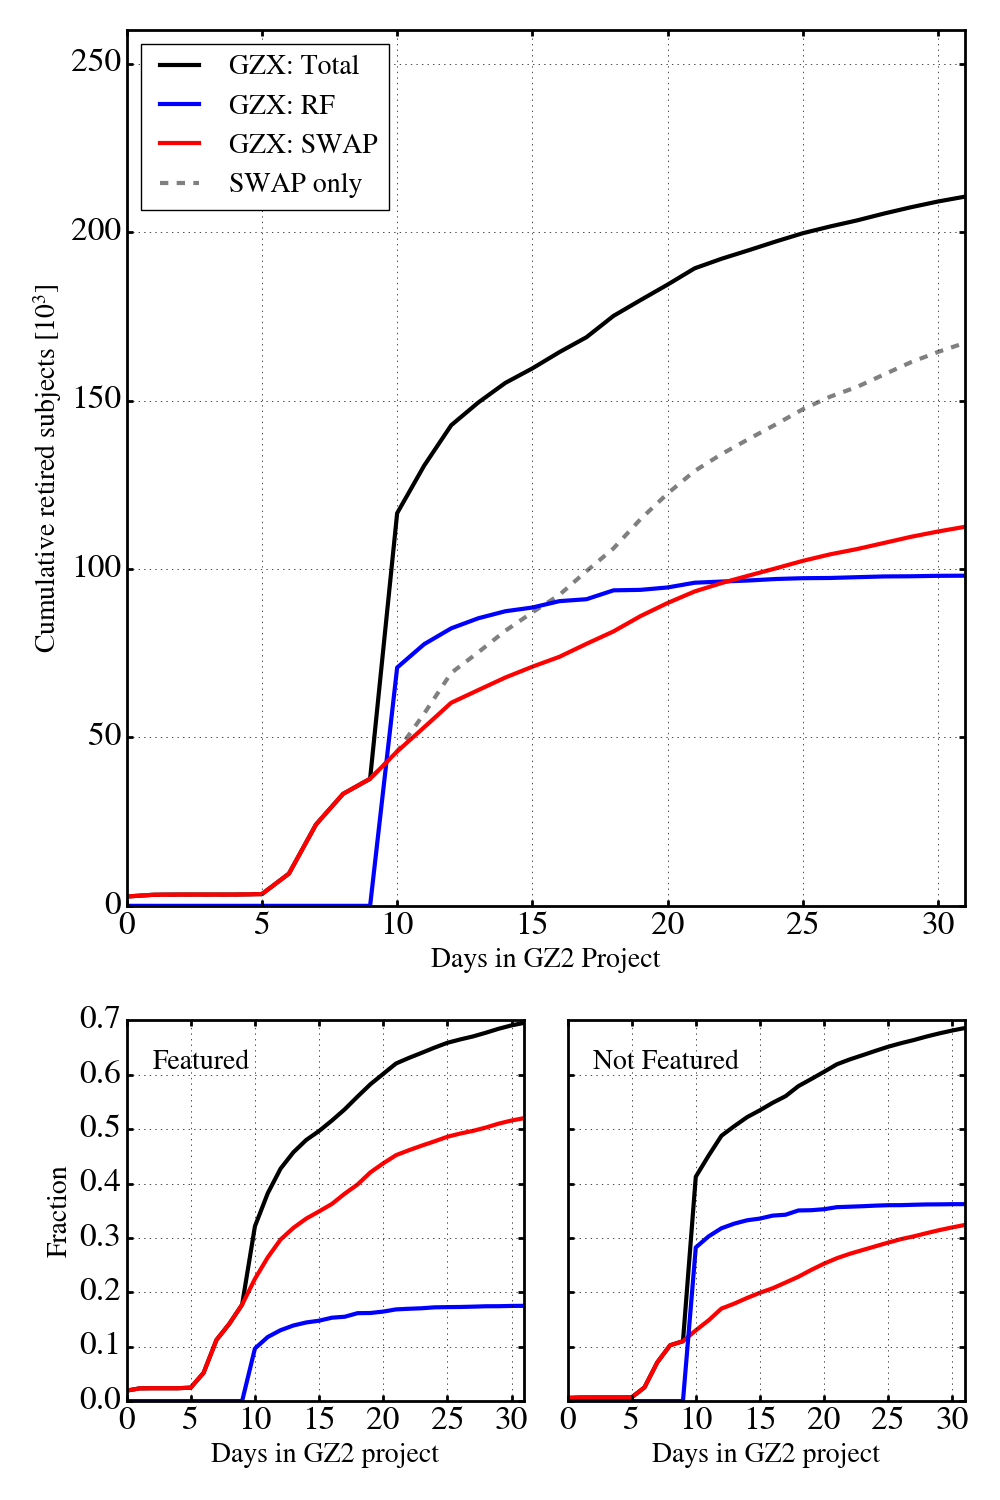
\includegraphics[width=3.3in]{figures/GZ2_sup_PLPD5_p5_flipfeature2b_RF_accuracy_redo_raw_combo_GZX_component_contributions.png}
\caption{The relative contributions of the human and machine components to the number of retired subjects are nearly equal but display very different behaviors over the course of our simulation (top panel). The bottom panel shows the total fraction of subjects retired split by class label. Overall, GZX retires over 70\% of the entire GZ2 sample in 32 days but the composition from each component is quite different. Humans retire more~\feat~subjects than the machine and vice versa. \label{fig: gzx components}}
\end{figure}

In the top panel of Figure~\ref{fig: gzx components} we explore the relative 
contribution to subject retirement from both the machine (blue) and SWAP (red). 
The solid black line shows the full GZX retirement 
and the dashed line shows the SWAP-only fiducial run from section~\ref{sec: fiducial}. 
Two things are immediately obvious. 
First, we see that, over the course of our simulation, the machine retires a total of 
$\sim100$K subjects while SWAP retires $\sim110$K subjects. Each shoulders approximately
half of the classification burden. Secondly, the behavior in the rates of these
retirements is clearly very different. Retirement through SWAP proceeds at a relatively
constant rate. In constrast, the machine contributes a surge in retirement during 
its first couple days, quickly overtaking the human contribution, but plateaus thereafter.
By Day 22, the human contribution through SWAP again becomes the primary mode 
of subject retirement. 


%%%-------------------------------------------------------
%%%  FIGURE:    MACHINE GETS IT RIGHT!!!
%%%-------------------------------------------------------
\begin{figure*}[t!]
\centering
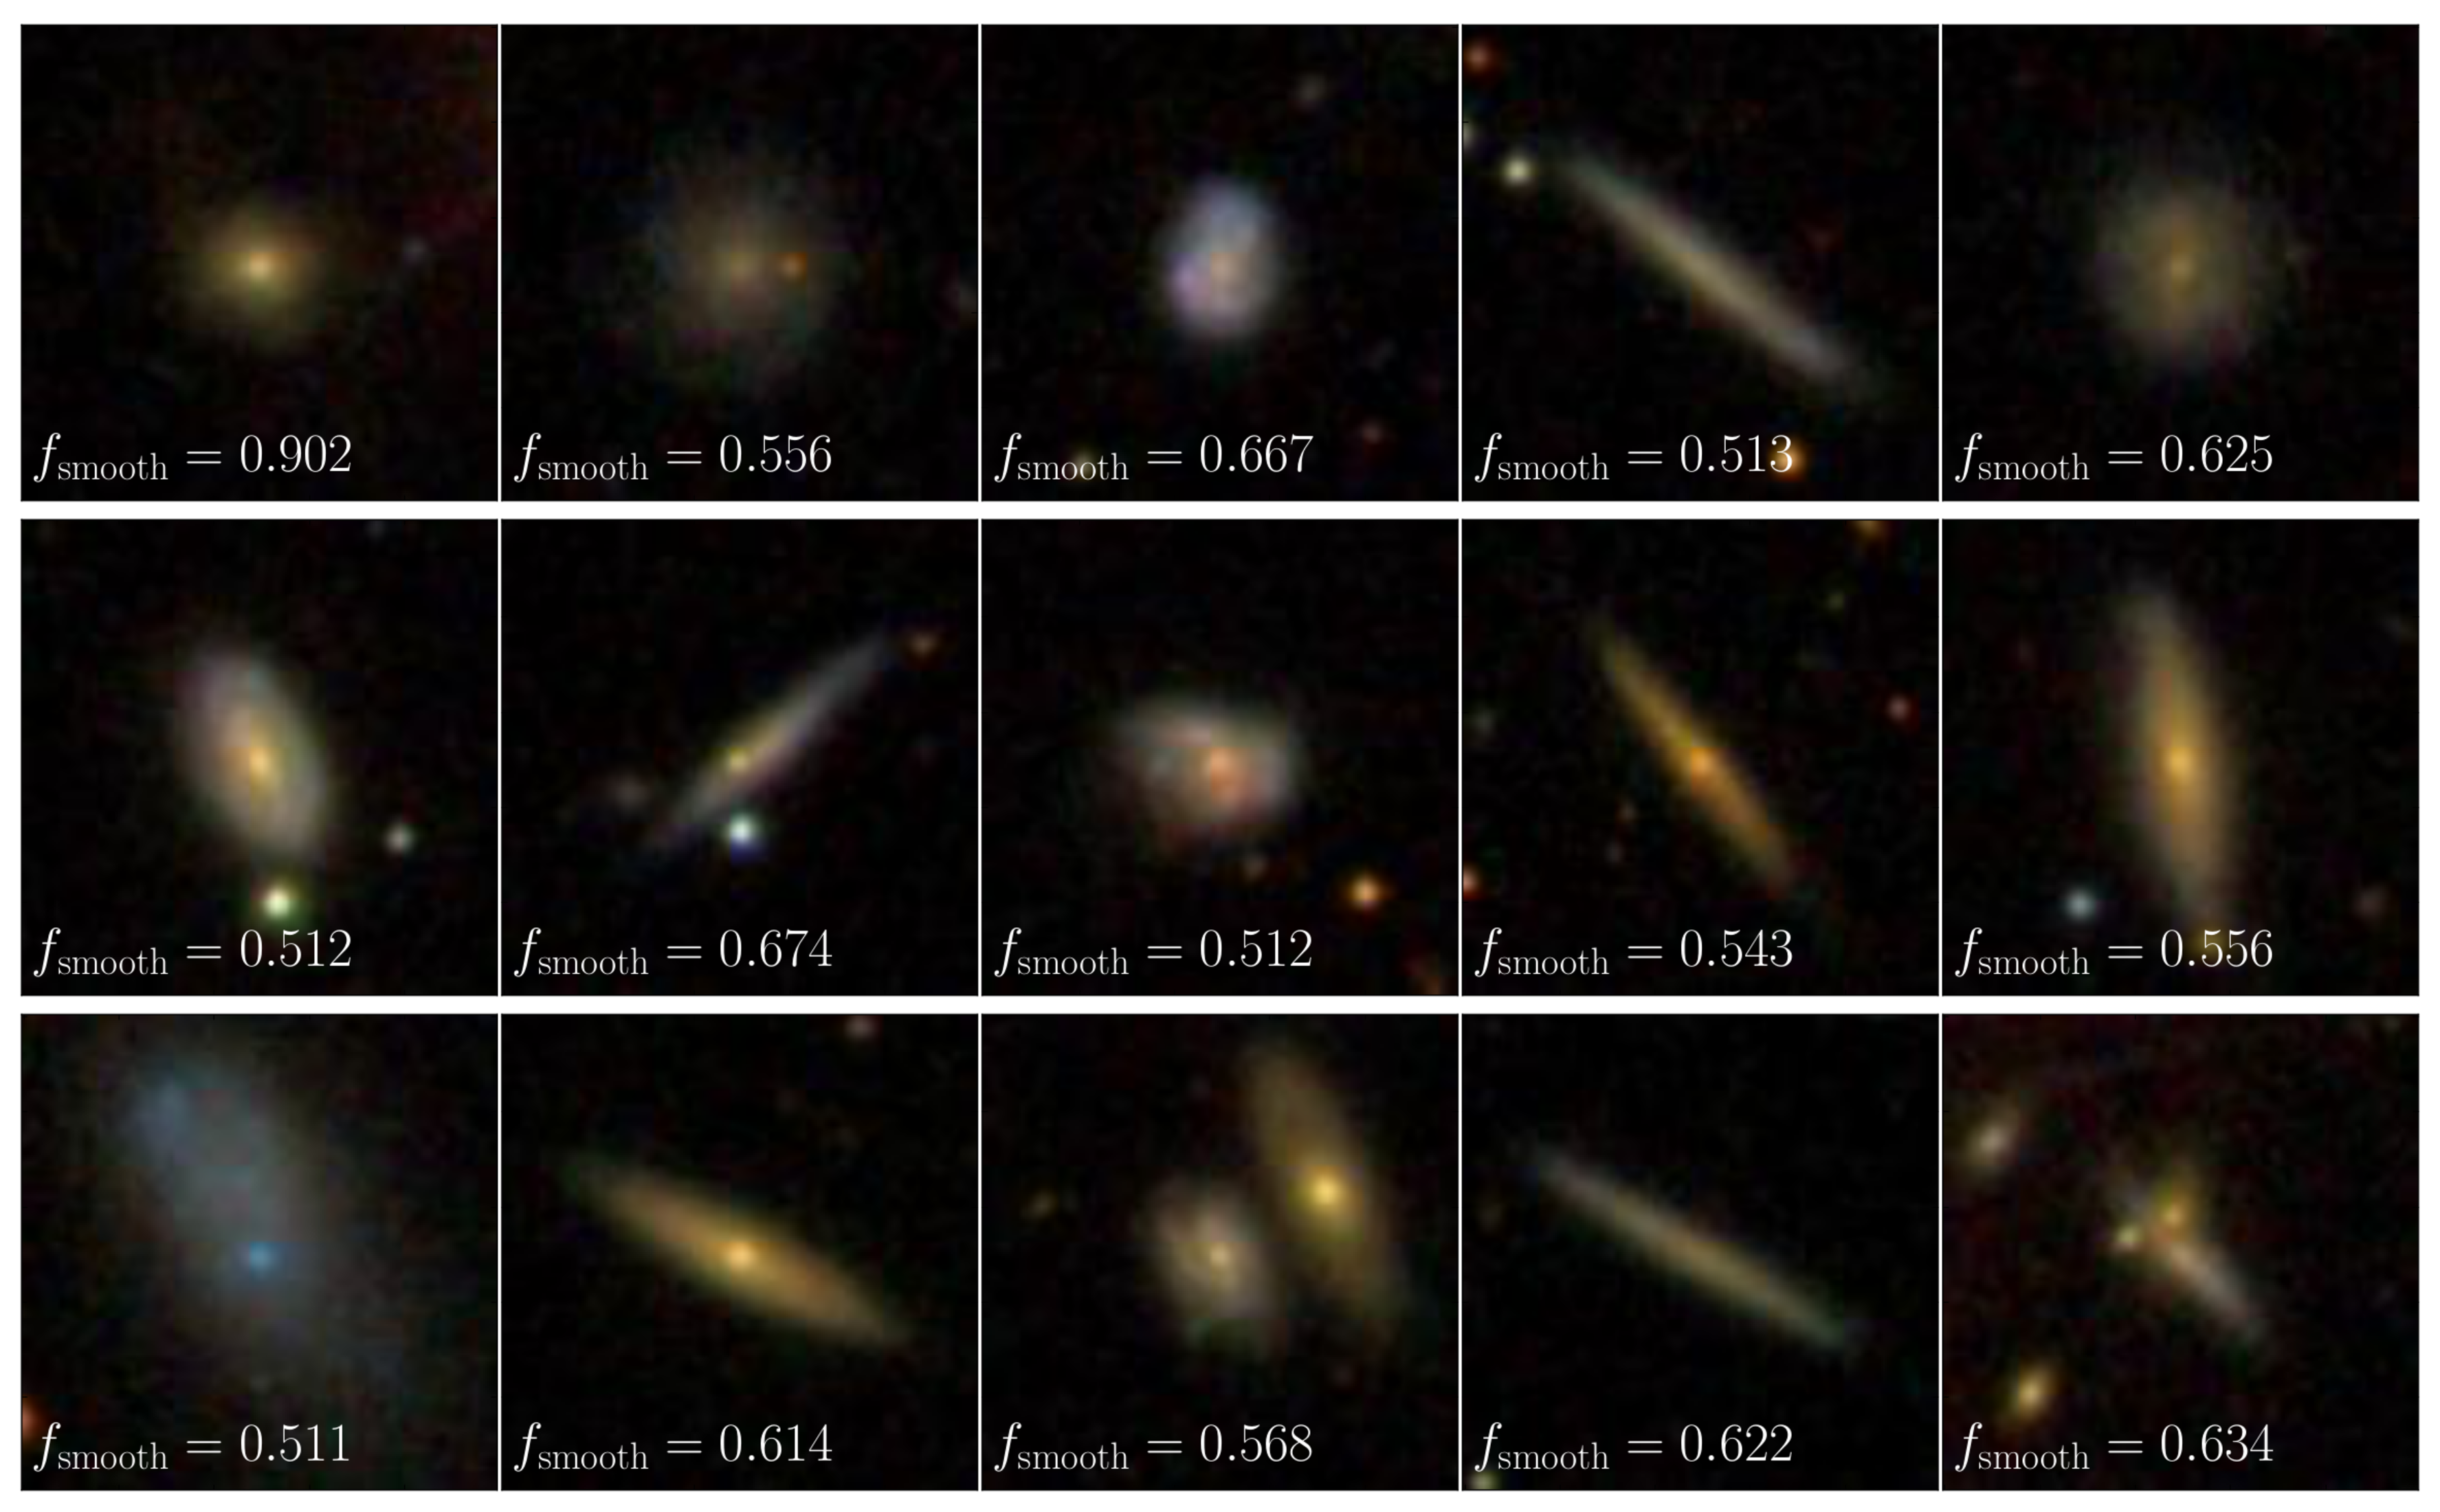
\includegraphics[width=6in]{figures/machine_false_positives_jpgs.png}
\caption{Galaxies the machine identifies as~\feat~but which the majority of human classifiers labeled as~\notfeat. The number in the lower left corner is the GZ2 smooth vote fraction, that is, the fraction of volunteers who classified the subject as `smooth'. These values are typically between 0.5 and 0.65 indicating that humans do not reach a strong consensus.  \label{fig: machine false pos}}
\end{figure*}

We thus clearly see three epochs of subject retirement, as we presumed.
In the first phase, humans are the only contributors to the total number of retired subjects.  
Once the machine has trained, it immediately contributes as much to subject retirement as humans.
However, the machine's performance plateaus faster than human performance;  the third 
phase of subject retirement is again dominated by human classifications.
% who again come to dominate the rate of subject retirement. 

Finally, we consider the composition of the two classifying agents in the bottom 
panels of Figure~\ref{fig: gzx components}. The left (right) panel shows the 
retired fraction of all subjects identified as~\feat~(\notfeat) as a function of project time. 
Over the course of the simulation, SWAP retires over 50\% of all~\feat~galaxies 
in the GZ2 sample while the machine retires only 18\%. Furthermore, this divergence 
only exists for~\feat~galaxies. In the lower right panel of  Figure~\ref{fig: gzx components}, 
we see that both humans and machine identify similar proportions (33-37\%) of 
the total number of~\notfeat~galaxies. 
%Of the subjects SWAP retires each night, 38\% to 40\% of them are 
%consistently and correctly identified as~\feat~culminating in the retirement of 
%over 50\% of the total number of~\feat~subjects in the GZ2 sample during the simulation. 
%In contrast, of the subjects retired by the machine, only 14\% of them are correctly 
%identified as~\feat~the first night the machine is run, increasing to only 20\% by 
%the end of the simulation. In total, the machine retires only 18\% of the total number
%of~\feat~subjects in the GZ2 sample.  

What is the source of this discrepancy? 
Why does the machine not identify with strong probability the remaining 30\% 
of~\feat~galaxies left unclassified by the end of our simulation? 
Are humans simply better at identifying featured galaxies with the machine optimized
to identify the~\notfeat~subjects? 
Each night the machine trains, it receives a training sample that is consistently composed of 30-40\%~\feat~galaxies, yet a similar proportion of~\feat~galaxies in the test sample
do not receive high $p_{machine}$.
Is this an artifact of our particular choice in machine, in the human-machine mechanism we've implemented here, or something else entirely?
In the next section we explore the machine's performance in the context of its 
training through human classifiers. 

\begin{comment}
This suggests that humans are optimized  to identify obviously~\feat~galaxies 
while the machine seems to identify the converse.
That humans and machine might be optimized  somewhat divergently is perhaps not 
unheard of when one considers that they are presented with different information 
and learn in entirely distinct ways. However,  the machine trains on a sample consistently
composed of 40\%~\feat~subjects provided by SWAP yet doesn't identify as many when 
applied to the test sample each night does deserve deeper consideration. 
In the next section we explore the machine's retirement to understand the core of its performance.
\end{comment}

\subsection{Machine performance}\label{sec: machine performance}

%%%%%%%%%%%% COMMENTED OUT %%%%%%%%%%%%%%%%%%
\begin{comment}
%%%-------------------------------------------------------
%%%  FIGURE:    MACHINE METRICS VARY WITH LABEL
%%%-------------------------------------------------------
\begin{figure}[t!]
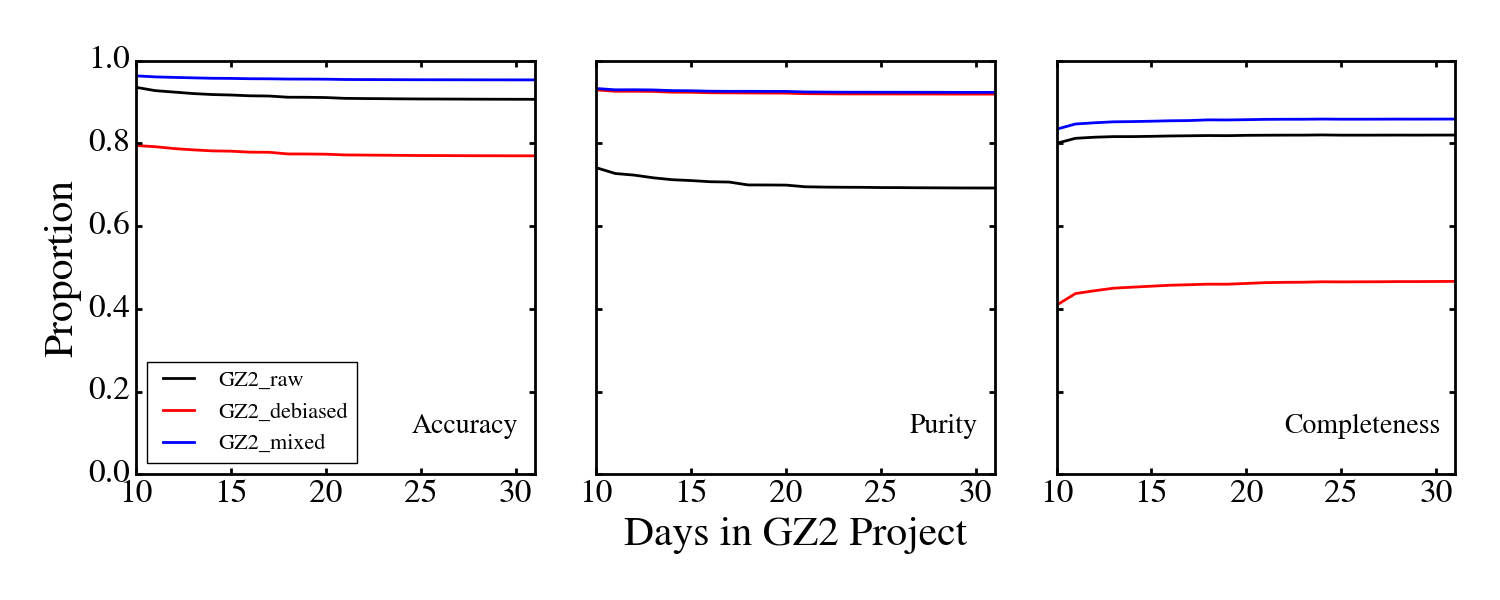
\includegraphics[width=3.5in]{figures/GZ2_sup_PLPD5_p5_flipfeature2b_RF_accuracy_redo_raw_combo_machine_metrics_comparison.png}
\caption{The performance of our RF algorithm varies depending on which set of GZ2 labels are provided as `truth'. Each panel shows the accuracy, purity, and completeness computed on the cumulatively retired subject set retired by that day in the simulation for three different sets of GZ2 labels: the raw vote fractions used throughout the analysis thus far, the debiased vote fractions, and a combination of the two described in the text. \label{fig: machine metrics}}
\end{figure}
\end{comment}


The analysis of the results thus far have assumed that~\raw~labels are ground
 truth for every GZ2 subject. These labels were the best choice to estimate the
quality of SWAP since we were directly comparing 
human consensus through two different aggregation algorithms.
However, the machine does not learn in the same way, nor is it presented with the 
same information. We argue that the machine classifications are, in fact, valid 
and complimentary to human classifications. 

We visually examine a portion of subjects that
were deemed false positives, i.e., galaxies retired as~\feat~by the machine which have~\notfeat~\raw~labels. 
Figure~\ref{fig: machine false pos} shows a random sample of images we inspected. 
The value in the lower left corner is the GZ2 smooth vote fraction, that is, the
fraction of volunteers who classified that subject as~\notfeat. The sample
consists primarily of edge-on disks and disk galaxies with low surface brightness
features. 

That the machine is apparently sensitive to a different information space and 
can identify~\feat~galaxies that humans classify as~\notfeat~likely has two 
 contributing factors: 
1) the first question of the GZ2 decision tree asks a very specific question; one which doesn't necessarily correlate with a split between early- and late-type galaxies, and 
 2) the machine learns on morphology diagnostics that are very different from visual inspection. 
% is a recognition that many humans will interpret a task quite literally, 
Regarding the first point, we see that GZ2 smooth vote fractions are generally
 between 0.5 and 0.65 for this sample indicating that volunteers have not 
reached a strong consensus. This behavior could be modified by providing
actual training images and live feedback as performed in \cite{Marshall2016}. 
The second point suggests that the morphology indicators we measure are 
sufficient for the machine to recognize~\feat~galaxies regardless of the labels humans provide. 
It remains to be seen whether this generalizes to other machine algorithms.
We note that most of these galaxies are labeled as~\feat~after GZ2's debiasing process. 

%In our system, the machine classifies subjects which are not seen by humans. However, the disagreement between human and machine is an area ripe for discovery. 
The complementary nature of human and machine classification can 
best be utilized by a feedback mechanism in which a portion of machine-retired
subjects are reviewed by humans. Subjects that display excessive disagreement
should be verified by an expert (or expert-user).  In the same way that 
humans increase the machine's training sample over time, subjects which the
machine properly identifies can become part of the humans' training sample. 
 
%%%%%%%%%%%% COMMENTED OUT %%%%%%%%%%%%%%%%%%
\begin{comment}
Figure~\ref{fig: machine metrics} examines the quality of the classifications made by 
the machine during the course of the simulation. The black lines represent our 
standard quality metrics computed from~\raw~labels. The red lines are the same 
metrics computed from~\deb~labels (themselves computed in an identical fashion
to the~\raw~labels described in section~\ref{sec: data}). It is immediately apparent
that different definitions of `truth' lead to significant variation in our quality metrics. 

We find the machine is identifying a subsample of galaxies that are 
labeled~\notfeat~according to~\raw~labels but are labeled~\feat~according to~\deb.
 This can be seen in the middle panel which shows the purity of~\feat~galaxies 
increases significantly when applying~\deb. This implies that
subjects considered false positives (labeled as~\notfeat~by~\raw) are truly~\feat~galaxies. 
We solidify this idea by computing the blue lines in Figure~\ref{fig: machine metrics}
wherein we apply~\deb~labels to the sample of false positives and~\raw~labels otherwise. 
The quality of the machine classifications improves in all categories. 

We see this explicitly by examining the morphology distributions for subsamples of
 machine-retired galaxies as shown in Figure~\ref{fig: morph params}.
 The top row shows the difference between these distributions for 
the~\feat~and~\notfeat~samples, while the middle row shows the false positive 
and false negative samples. We see that the morphology distributions for the 
false positive sample are nearly identical to the morphology distributions for the~\feat~sample. 

Why then doesn't the machine identify all galaxies that are ultimately
labeled as~\feat~by~\deb~labels? We know it does not as evidenced by the paltry
42\%~\deb~completeness displayed in the right-most panel of Figure~\ref{fig: machine metrics}.
This is likely a consequence of the machine training on labels provided by SWAP 
which match~\raw~labels to 95\%. We would expect a higher level of completeness
 if we instead provided the machine with debiased labels. 

The machine is retiring more~\feat~galaxies than~\raw~labels suggest but not all that 
the~\deb~labels suggest. 

%%%-------------------------------------------------------
%%%  FIGURE:   CAS DISTRIBUTIONS 
%%%-------------------------------------------------------
\begin{figure*}[t!]
\centering
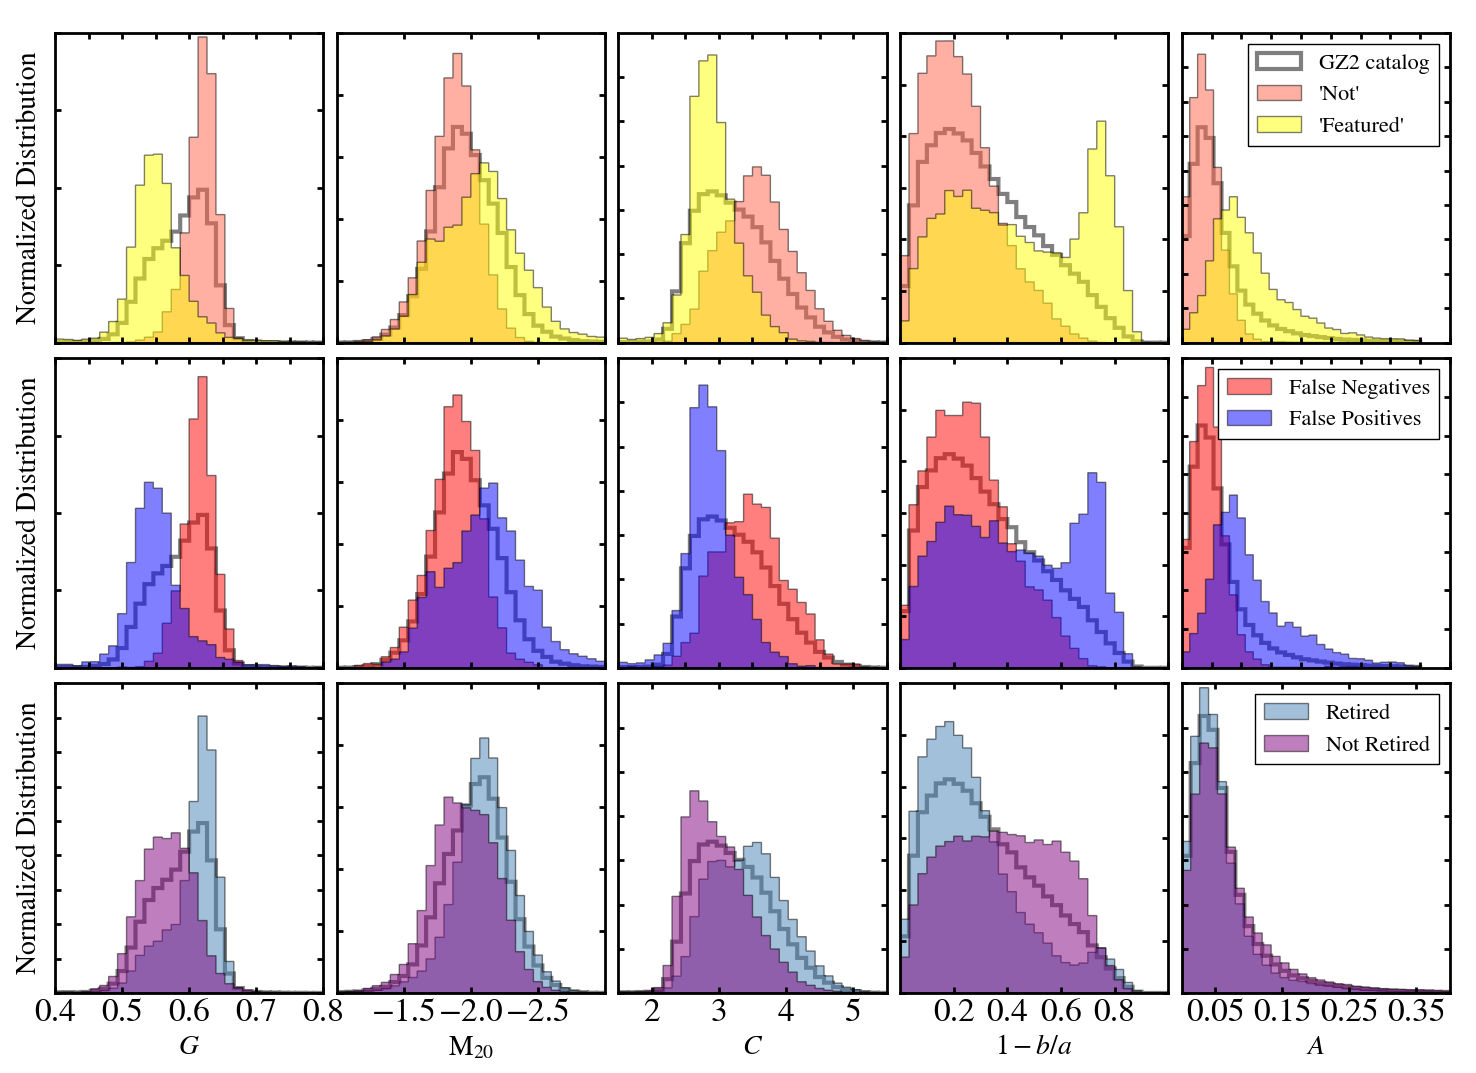
\includegraphics[width=7in]{figures/GZ2_sup_PLPD5_p5_flipfeature2b_RF_accuracy_redo_raw_combo_morph_params_raw_labels_4paper.png}
\caption{What the machine can and can't classify. \label{fig: morph params}}
\end{figure*}

\end{comment}
%%%%%%%%%%%%  END COMMENT %%%%%%%%%%%%%%%%%%


%It is well known that visual classifications are sensitive to a galaxy's redshift and surface brightness. For this reason,~\cite{Willett2013} compute corrections to the volunteer vote fractions. These debiased vote fractions effectively increase the number of~\feat~galaxies in the GZ2 sample. 

%However, we surmise that the machine is not biased in the same way. It receives  a 5 dimensional morphology parameter space  which is very different from the much higher dimensional space of a color jpeg that humans see. However, these parameters are specifically known to correlate with various galaxy morphology properties in a predictable way. For example, galaxies with very high ellipticity are predominantly edge-on and would thus fall under the~\feat~category, while galaxies with high concentrations would suggest they belong to the~\notfeat~category.  More importantly, the efficacy of these parameters is not heavily dependent on the redshift range of the GZ2 galaxy sample \textbf{[citations]}. Thus, these parameters provide a less-biased feature space which suggests that the GZ2 vote fractions we computed before might not hold in all cases.

%We can see evidence for this by considering how the quality metrics we compute for the machine's performance vary when comparing the output to different GZ2 `truth' labels. Figure~\ref{fig: machine metrics} shows our standard quality metrics but now considering only the subjects which the machine retires. The black lines show the machine's performance when using the GZ2 raw vote fractions as done previously. The red lines are the performance when using the GZ2 debiased vote fractions. This has the effect of dramatically increasing the purity of the sample (fewer~\notfeat~subjects contaminate the sample) but the completeness (how many~\feat~we recover) drops significantly. This might seem to be evidence to the contrary but we note that the GZ2 debiasing technique affects a full third of the galaxies in the GZ2 catalog. Since the machine is not trained on these labels, it doesn't recover the significantly increased fraction of~\feat~galaxies. Finally, we construct a mix of these two labels in the following way: Under the assumption that the machine is identifying more~\feat~subjects than it seems, we look at the group of false positives, those subjects which the machine identified as~\feat~but which the GZ2 raw labels claimare~\notfeat. To this subset we apply the GZ2 debiased label and the results are shown in blue. All metrics improve dramatically and are, in fact, better than either individual set of labels. 


%for each of the five morphology parameters on which the machine trains.  
%Furthermore, if we instead plot those labeled as false positives 
%according to their GZ2 debiased label, the sharp peak in the ellipticity distribution 
%disappears entirely. 
%Finally, the bottom row shows the distributions of all machine-retired
%subjects with those which the machine did not retire, i.e., those where the machine 
%predicted labels with $p_{machine}<0.9$. The distribution of those not retired by the machine
%display properties of both~\feat~and~\notfeat~as evidenced by a broader Gini and
%Concentration distributions. 
%Though these two distributions seem to be more similar
%to the distribution of~\feat~subjects, the lack of obvious peak in the ellipticity distribution 
%could indicate that the machine needs at least 3 parameters to strongly predict a~\feat~label.


%Another desirable quality of the RF algorithm is its interpretability. The trees in the forest each split on values for every dimension of the feature vector where  splits that reduce the prediction error are preferred. From this one can reconstruct which features are most important for determining class predictions. Unsurprisingly, our machine puts a great deal of weight on the Gini coefficient which is clearly evident in the decisive separation between subject subsets  in the top two rows of Figure~\ref{fig: morph params}. The RF next places nearly equal weight on Concentration and ellipticity.  \textbf{double check this and values}

%We recognize that deep learning algorithms are becoming increasingly popular and incredibly powerful at accurate prediction. However, a core drawback to these algorithms is their black box quality. Not only is it difficult to interpret which features they identify, it has yet to be shown how or if these features directly relate to the physical  properties of galaxies. Furthermore, while huertas-company, deilman ( and others?) have demonstrated that these algorithms can be trained to very accurately predict just as humans would, we know that human classification is inherently biased (moreso for the general public, but even experts disagree!). By using a simple off-the-shelf random forest we may not achieve the same level of accuracy as a deep learning algorithm, however we argue this is due to the fact that this machine can be optimized to, in a sense, counteract human bias. 

%The motivating goal behind GZX is to provide a practical framework to increase the rate of galaxy morphology classification without sacrificing the quality of those classifications. We thus advocate that one should use their machine of choice in place of a RF if so desired. This choice should be motivated by the science goals of the project. 

%Indeed, the original GZ2classifications were never intended 
%to be used directly as a catalog. The authors strongly urge cuts down the decision tree as
%as well as in magnitude and redshift. 

%We examine in the size-magnitude plane those  subjects retired by machine as shown in Fig~\ref{fig: machine classified}.  We see see the first classification by the machine includes a healthy mix of both `Featured` and `Not' subjects over a broad range of magnitude and sizes. These subjects are "easy to classify" as they are large and bright. However, by the end of the run the machine (combined with SWAP) have classifed the easiest subjects; those with the most information stored in their images.  On the last day we peform the simulation, the machine is only classifying small, faint  subjects; all the larger and brighter subjects have been retired. Small, faint subjects are notoriously difficult to classify. As such, when comparing the resulting prediction from the machine to the original label provided by GZ2, it is less likely that machine matches that prediction. Indeed, it is just as likely that the original GZ2 classifications are inherently wrong themselves. \textbf{Show a random sample of original jpg images? } 


%%----------------------------------------------------------------------------------------------------------------------------------------------------
%%   MAD RAVINGS OF THE FUTURE 
%%----------------------------------------------------------------------------------------------------------------------------------------------------
\section{Looking Forward}\label{sec: visions}

We have demonstrated the first practical framework for combining human and machine
 intelligence in galaxy morphology classifications tasks. 
%By reprocessing the original Galaxy Zoo 2 classifications with SWAP, incorporating a supervised machine learningalgorithm, and implementing a simple decision engine which guides how these two agents interact, we achieve an order of magnitude increase in the classification rate. 
%This is achieved while maintaining accurate identification of both~\feat~and~\notfeat~
%galaxies to over 95\%. Additionally, we recover nearly 95\% of~\feat~galaxies with contamination at a modest 15\%. We now discuss our road map for the future including implications for upcoming massive surveys such as LSST or Euclid. 
Our results have implications for the future of citizen science in general and 
Galaxy Zoo in particular, however we focus instead on a brief discussion of our next 
steps and potential applications to large upcoming surveys. 

%\subsection{From Simple to Sophisticated}
GZX represents perhaps one of the simplest ways to combine human
and machine intelligence. Its impressive performance motivates a higher 
level of sophistication. We presen tthree of the most 
straightforward steps that will advance our system to the next level, implementation
that will improve both the rate of quality of morphology classifications. 

First, our current system contains only a passive feedback mechanism. However,  
we envision multiple forms of active feedback.  SWAP allows us to leverage the 
most skilled volunteers to review those galaxies which are the most difficult for either
 human or machine classify. Additionally, a portion of subjects classified by machine 
should subsequently be reviewed by humans since we have shown that disagreements 
between these two agents could signify to experts that something interesting is afoot. 

%This could additionally provide a timely warning: if the machine consistently fails the spot-checking, a new algorithm could instead take its place. as a means of spot-checking that the machine is performing as expected as well 

Secondly, the random forest algorithm is not easily adapted to handle measurement 
errors or class labels with continuous distributions. To fully utilize the information provided by
SWAP, algorithms which can handle continuous distributions for the input and output 
subject labels should be explored. 
These include deep convolutional neural networks (CNN) or Latent Dirichlet allocation (LDA), 
an algorithm that is frequently used in document processing. 

%That being said, a RF is still a very simplistic machine.
% It is highly sensitive to outliers in the feature vector space. It cannot accept measurement error on features. And it can only accept distinct class labels 
%(though it can certainly handle more than 2 as we have done here!). 
%One way to better utilize all available information would be to 
%implement an algorithm that could accept a continuous distribution as a label which 
%this is precisely what SWAP outputs for every subject. Furthermore, providing a 
%probability distribution of possible output labels would also be wise as there are 
%galaxies that exhibit both~\feat~and~\notfeat~properties.
%Galaxy morphology is only distinct at the far ends of the spectrum with a great 
%many subjects wading in the middle, exhibiting a mixed set of features. Luckily, 
%It is already known that CNNs can accurately predict 
%galaxy morphology labels but application of LDA to this type of task has never 
%been attempted, to our knowledge. 

%We have demonstrated that dramatic results can be gained using a simple random forest algorithm. This machine has several desirable qualities. One can understand the machine's performance directly by examining the distribution of output in each of the input features as we have done in section~\ref{sec: machine performance}. Thus one can monitor that performance and make further decisions based on it (does the machine need additional training? should a different machine be used? etc.). Secondly, this algorithm can inherently output probabilities associated with each prediction and identify which features were most important to that prediction. Finally, this machine is very fast to train. Even with a considerable cross-validation, the RF can train on 75K subjects in under and hour with an 2.9GHz 8-core laptop. 

%\textbf{A larger feature vector for each subject.} 
%Our choice of feature vector stems from work on ZEST~\citep{Scarlata2007} who used the same set of features in a Principal Component Analysis to classify 120K galaxies in the COSMOS field. Though G, M20, C, A, e have been well studied for decades and known to correlate with physical properties of galaxies. There are additional morphological parameters that correlate with galaxy properties which a machine algorithm could find more informative than the features we provide here.  In particular, the MID statistics of~\cite{Freeman2013} have been shown to correlate well for higher redshift galaxies and are less sensitive to noise. Our current features coupled with the MID statistics are all non-parametric indicators and could easily be implemented as basic measurements in upcoming survey reduction pipelines. Additionally, information could be gained by the inclusion of parametric features such as  Sersic index and bulge to total ratio, though these are more time consuming to measure in bulk. 

%We note that the morphology indicators we have discussed so far are geared towards  distinguishing between early- and late-type galaxies. However, our framework is applicable  to far more than just~\feat~or~\notfeat. A different question would require a  set of  features that appropriately identify the morphology of interest. It is well known in machine-learning circles that choosing an appropriate feature vector is more of an art than a science, thus these choices should be tested on a  subsample prior to implementation in GZX. 

%\textbf{A larger confusion matrix for SWAP.}
%The core of SWAP revolves around the confusion matrix that an agent assigns to each
%volunteer. Extending the confusion matrix to three dimensions should be relatively 
%straightforward and would allow for more detailed morphology tasks.
%We note that most questions in the Galaxy Zoo decision tree could be easily modified
%to consist of three responses.
%Higher dimensions than this will quickly grow in complexity without much in additional gain. 

%Our simulations considered a binary classification task as this is how SWAP was originally built. It was created with the goal of identifying rare events to which it was only necessary to ask if the image in question contained a gravitational lens or not. We have demonstrated that SWAP can be used for pure classification and for a task which is perhaps the most common question in the local Universe. And though much can be gained from simple binary tasks, there will always be occasion for a more complex classification. Specifically, any morphology task concerned with the strength of a feature (i.e., How pronounced is the galactic bulge, if one exists?) will be difficult to force into a binary box. 

Finally, we envision another instance of SWAP to aggregate an ensemble of machine classifiers in a similar fashion to the human counterparts as hinted at in Figure~\ref{fig: schematic}.
In this scheme, several disparate machine algorithms could train simultaneously 
on the same training sample with their predictions aggregated through SWAP. 
%We have already implemented an agent which is assigned to our machine classifier. This agent tracks the machine's performance over time and could, in principle, be used in exactly the same way as agents assigned to human classifiers. 

%There is much work in the machine learning community concerning ensemble algorithms \textbf{[citations?]} and, in fact, a Random Forest is such an algorithm. These types of algorithms, and RF specifically, are created to reduce variance (sensitivity to small fluctuations in the training set) without increasing bias (error induced by erroneous assumptions in the learning algorithm, i.e., missing relevant relations between features). It remains to be tested whether SWAP aggregation of a group of machines algorithms  will yield similar fruit. 

%\textbf{Classifications are not debiased.}  
%It is a known issue that any visual classification will be biased by several effects, especially redshift and size. Lack of depth and resolution at higher redshift tend to produce classifications which lack observable features. Galaxy Zoo 2 is able to account for redshift bias by adjusting the vote fractions produced by the volunteers. This step is done after the fact by considering for every Galaxy Zoo catalog  \cite{Willett2013}, \cite{Willett2016}, \cite{Simmons2016}.  Throughout this paper, we compare predicted classes to a majority raw GZ2 vote fractions. These vote fractions are not corrected for redshift bias. As states above, we chose these vote fractions because SWAP processes the original votes and does not have functionality to debias these votes. Thus, this step must still be done after subjects are retired or the project completes. 

%\textbf{Low redshift regime -- what can we do for higher z data?}
%GZ2 is a low redshift sample of galaxies, those to which the Hubble tuning fork could be applied. At higher redshift, these class labels break down.  Similarly, standard methods of quantifying morphological structure also suffer as M20 and Gini coefficient are susceptible to noise (I think, cite XXX). Additionally, as the shapes of galaxies are significantly different at higher redshift, different metrics of morphology would be more appropriate. We could easily extend our machine to perform on high redshift samples by incorporating the MID statistics \ref{Freedman2013}. Another future test will be to examine how GZX performs on Galaxy Zoo: Hubble and Galaxy Zoo: CANDELS datasets. 


\begin{comment}
%%----------------------------------------------------------------------------------------------------------------------------------------------------
%%  VISIONS FOR CITIZEN SCIENCE
%%----------------------------------------------------------------------------------------------------------------------------------------------------
%\subsection{Visions for Citizen Science}
The work presented here has provided us with unprecedented insight into the Galaxy Zoo project and, by extension, citizen science projects. Here we present a few of our thoughts and suggestions for maximizing the wisdom of the crowd. 

%\textbf{Don't waste volunteers' time.} A core tenant of the Citizen Science Alliance (?)/
citizen science 
 is not wasting human effort. If a project can be accomplished by a small 
group of experts, by an automated task, or a combination of both, citizen scientists
should not be tapped. SWAP alone presents a means to reduce the required 
effort from citizen scientists by a factor of 4-5. After incorporating a machine, we 
reduce human effort by XXX. Human eyes thus remain crucial to classification tasks
as training samples don't generate themselves, but the burden can and should be reduced. 

Towards that end, the Zooniverse has plans and is currently developing
several of the techniques presented here into their online platform. Though we 
note that our framework doesn't necessarily require Galaxy Zoo or the Zooniverse, 
it is the largest citizen science web platform in the world. Once SWAP has been
implemented on their back end, they are an obvious choice for handling at least
the crowd-sourcing aspect of classification tasks. 
\textbf{[Chris: feel free to adjust/add/subtract from this section as you see fit!]}


%\textbf{Engagement = More votes = faster classification.}
Nearly every Zooniverse project has a surge of volunteer effort within the first 
few days of a project's inception. The results we present here are due in large 
part to this phenomenon. If one looks at the rate of incoming volunteer classifications
for the original Galaxy Zoo 2 project, it peaks on day 2-3 at over 400K! Within one
week of GZ2's inception, XXX classifications were made by XXX volunteers. 
 After the initial excitement dies down, most projects receive
a greatly reduced but steady stream of classifications. Therefore, take advantage
 of this initial peak in classifications by generating excitement with emphasis on 
volunteer engagement. This leads to a greater the surge in volunteer classifications 
at the outset of a project, and allows SWAP and the machine to tackle substantial data sets.  


%\textbf{Train your volunteers.}
The Space Warps Zooniverse project was one of the first citizen science projects
to demonstrate that humans could be trained in a similar way as machine algorithms, 
and that this effect could be substantial and quantified.  Although we have strived to 
mimic this process, we obviously could not provide feedback in real time. We have, 
however compared the classifications of the top 5 most skilled GZ2 volunteers
(as quantified by SWAP) to our expert classifications for the sample of 3500 galaxies 
we described in section~\ref{sec: training sample}. We find that even the most
skilled volunteers are still biased towards classifying galaxies as~\notfeat.
We surmise this is due, in part, to the fact that GZ2 did not provide a training 
program which precluded volunteers from discerning S0-Sa galaxies, a task at 
which experts are more sensitive.  

Applications of GZX to other projects will require PIs to develop appropriate 
gold standard samples for their data. We suggest that this expert sample could be
developed using the Zooniverse Project Builder, an open source, free to use, web based 
service which allows science teams to build and classify their own data.
 How large should the sample be?  Unfortunately, this question is outside the scope 
of this paper. However, our sister publication~\citep{Wright2016, submitted}, uses 
SWAP in a live project classifying XXX and discusses the 
%Alternatively, the first question in Galaxy Zoo could be reworded to exclude the concept of `disk' which is never explained. 


%\textbf{Decision Trees versus Volunteer Experience}
Every iteration of Galaxy Zoo, with the exception of the the original project, has 
adopted a decision tree yielding dozens of possible class labels from several tasks.
The downside to this structure is the complications arising in both aggregation of  
volunteer votes and the ease of which one can use the resulting GZ catalogs. True 
statistical samples cannot be created because the same questions are not asked 
of every subject. GZ catalogs can be used to identify pure samples at the expense
of completeness, where these samples are generated through a series of cuts on 
every task in the decision tree preceding the question of interest. 

Our vision for the future of Galaxy Zoo and other projects which utilize decision trees
would have an instance of SWAP for each task in the tree and, if appropriate, 
one or several machine classifiers.  The volunteer would still see a sensible subsequent
question depending on her response but SWAP would appropriate a negative response 
for every subsequent task down the path she doesn't take. For example, 
if she answered~\feat~to the first question, SWAP would automatically record a 
negative response to every subsequent question down the `Smooth' path of the decision tree. 
This would allow every subject in the sample to receive an answer for every question
 in the decision tree thus providing statistical reliability, easier vote aggregation analysis, 
and straightforward data products.  

This would require additional SWAP architecture such that a single agent assigned
to a volunteer would have the additional directive to participate in several instances of SWAP
at once, where that volunteer is assigned as many confusion matrices as questions in the tree.
These suggestions are motivated, in part, due to observed volunteer experience. 
 Separating the decision tree into several distinct tasks has been shown to fall short 
in compelling volunteers to carry on the project \textbf{[Chris: citations? comments?]}. 
It seems volunteers prefer more integrated tasks. This is 
important because it relates to engagement which in turn can encourage additional
volunteers and classifications as discussed above. 
\end{comment}

%%----------------------------------------------------------------------------------------------------------------------------------------------------
%%  IMPLICATIONS FOR UPCOMING LARGE-SCALE SURVEYS
%%----------------------------------------------------------------------------------------------------------------------------------------------------
%\subsection{Dealing with the Data Deluge}
%The work in this paper is motivated by the need for increased speed in the face of several large surveys coming online in the next 5 years. These projects promise to deliver more raw data per night than we have accumulated in the past  decade. Though these efforts are concentrated on probing dark energy, we briefly discuss how GZX might handle the data deluge to maximize the science output of these surveys.

%\textbf{Is an order of magnitude enough?} 
%We've demonstrated that we can achieve an order of magnitude increase in the rate of subject retirement for galaxy morphology tasks. Is this enough?  
With the above upgrades implemented, we expect performance of both the
classification rate and quality to increase. However, even with our current 
implementation we can envision coping with the upcoming data deluge. 
By some estimates, Euclid is expected to obtain
measurable morphology with VIS for approximately $10^6 - 10^7$ galaxies.
Traditional visual classification at the rate achieved today through Galaxy Zoo 
would require approximately 300 years to classify such a large dataset. 
GZX as currently implemented could  classify the brightest 20\% of the full 
Euclid sample within the six years of its observing mission. 
We predict this is a lower limit as more sophisticated machine learning algorithms
will undoubtedly be capable of further efficiency. 
%Our method would allow us to classify At the current rate of  Galaxy Zoo is currently able to classify roughly 400 images per day. At that rate, it would take over 3000 years
%to classify the entire Euclid sample.  

%The Euclid collaboration is already considering which morphology indicators will
%be built into their reduction pipeline for galaxy morphology studies and we suggest
%that LSST do likewise \textbf{[Are they already?]}. 
%Not only are these suitable for galaxy studies themselves, 
%they provide the framework and feedback by which we can judge a machine classifier's 
%performance. 

%\textbf{Is the performance enough?} 
%As currently implemented, we can obtain accuracy around 95\%. That could leave us with hundreds of thousands of galaxies with unreliable classifications. Such a dataset will provide a wealth of information for a slew of science cases, however, to extract the most from these datasets, additional gains in performance may be required. One solution is to incorporate deep learning algorithms which can provide higher quality classifications at the expense of interpretability. Ensembles of machine classifiers aggregated through SWAP could provide another promising avenue. A third solution is presented in our sister publication (Wright et al. 2016, submitted) whereby accuracy is dramatically increased through an entirely different human-machine combination. In that paper we explore the effects of averaging the human and machine classification scores and find that the combined score yields the most reliable classification. 




%%----------------------------------------------------------------------------------------------------------------------------------------------------
%%   CONCLUSIONS 
%%----------------------------------------------------------------------------------------------------------------------------------------------------
\subsection{Conclusions}

We test a novel system for the efficient classification 
of galaxy morphology tasks that integrates the native ability of the human 
mind to identify the abstract and novel with machine learning algorithms which provide
 speed and brute force.  

We demonstrate for the first time that the SWAP algorithm, 
originally developed to identify rare gravitational lenses in the Space Warps project, 
is robust for use in galaxy morphology classification. We show that by implementing
SWAP on GZ2 classification data we can increase the rate of classification by a factor
of 4-5, requiring only 90 days of project time to sufficiently classify nearly 80\% of the
entire GZ2 galaxy sample. 

Furthermore, we have implemented and tested a simple Random Forest algorithm 
and developed a decision engine that delegates tasks between human and 
machine.  We show that even this simple machine is capable of providing significant 
gains in the rate of classification allowing us to retire over 70\% of GZ2 galaxies in 
just 32 days of GZ2 project time, representing an order of magnitude increase in the
classification rate compared to the original Galaxy Zoo 2 project. This is achieved without 
sacrificing the quality of classifications as we maintain accuracy well above 90\% 
throughout our simulations. 
Additionally, we have shown that training on a 5-dimensional parameter space of 
traditional non-parametric morphology indicators allows the
machine to identify subjects which humans miss, providing  a complementary 
approach to visual classification. 
The gain in classification speed allows us to tackle the massive amounts of data soon
to be forthcoming from large surveys like LSST, Euclid, and WFIRST. 
%With a few modest upgrades to our GZX framework we are confident this method will be able to handle the gargantuan task of morphology classification of the billions of galaxies soon to be cataloged. 



%%----------------------------------------------------------------------------------------------------------------------------------------------------
%%   ACKNOWLEDGEMENTS
%%----------------------------------------------------------------------------------------------------------------------------------------------------
\section{Acknowledgements}
MB thanks John Wallin, Steven Bamford, and Boris H{\"a}u{\ss}ler for discussions which helped elucidate things and stuff. 

MB, CS, LF, KW, and MG gratefully acknowledge support from the US National Science
Foundation Grant AST1413610.  MB acknowledges additional support 
through New College and Oxford University's Balzan Fellowship as well as the University
of Minnesota's Doctoral Dissertation Fellowship. Travel funding was supplied 
to MB, in part, by the University of Minnesota's Thesis Research Travel Grant. CJL recognizes support from a grant from the Science \& Technology Facilities Council (ST/N003179/1). 





%%----------------------------------------------------------------------------------------------------------------------------------------------------
%%   APPENDIX
%%----------------------------------------------------------------------------------------------------------------------------------------------------
\appendix
\label{sec:Appendix}

\section{Measuring Nonparametric Morphological Diagnostics on SDSS Stamps}
\label{sec: measuring morphology}

We obtain $i$-band imaging from SDSS data release 12. Postage stamps are made from the SDSS fields for each galaxy with dimensions of 3 Petrosian radii. Galaxies located within 3 Petrosian radii of the edge of a field were excluded.  Postage stamps undergo a cleaning process whereby nearby sources are identified with SExtractor \citep[ver. 2.8.6;][]{sextractor} and their pixels replaced with values that mimic the background in that region. We compute the following widely adopted nonparametric measurements  of the galaxy light distribution on the cleaned postage stamps:


Concentration is computed as $C = 5\log(r_{80}/ r_{20})$ where \rr{80} and \rr{20} are the radii containing 80\% and 20\% of the galaxy light respectively.  Large values of this ratio tend to indicate disky galaxies, while smaller values correlate with early-type ellipticals. 

Asymmetry quantifies the degree of rotational symmetry in the galaxy light distribution (not necessarily the physical shape of the galaxy as this parameter is not highly sensitive to low surface brightness features). A correction for background noise is applied (as in e.g.~\cite{Conselice2000}), i.e., 
\begin{equation}
A = \frac{\sum_{x,y} |I - I_{180}|}{ 2\sum|I|} - B_{180}
\end{equation}
where $I$ is the galaxy flux in each pixel $(x, y)$, $I_{180}$ is the image rotated by 180 degrees about the galaxy's central pixel, and $B_{180}$ is the average asymmetry of the background. 

The Gini coefficient, $G$,~\citep{Glasser1962, Abraham2003} describes how uniformly distributed a galaxy's flux is.  If $G$ is 0, the flux is distributed homogeneously among all galaxy pixels.; if $G$ is 1,  the light is contained within a single pixel. This term correlates with $C$, however, $G$ does not require that the flux be in the central region of the galaxy.  We follow~\cite{Lotz2004} by first ordering the pixels by increasing flux value, and then computing
\begin{equation}
G = \frac{1}{|\bar X|n(n-1)}\sum_i^n(2i-n-1)|X_i|
\end{equation}
where $n$ is the number of pixels assigned to the galaxy, and $\bar X$ is the mean pixel value. 

\M{20}~\citep{Lotz2004} is the second order moment of the brightest 20\% of the galaxy flux. We compute it as
\begin{eqnarray}
 M_{tot} & = & \sum_i^nf_i[(x_i-x_c)^2 + (y_i-y_c)^2]  \\
 M_{20} & = & \log_{10} (\frac{\sum_iM_i}{M_{tot}}), ~~\textrm{while} \sum_ifi < 0.2f_{tot}
\end{eqnarray}
where M$_{tot}$, the total moment, is computed first and $f_{tot}$ is the total flux. For centrally concentrated objects, \M{20} correlates with $C$ but is also sensitive to bright off-center knots of light. 

Finally, we use the ellipticity, $\epsilon = 1 - b/a$, of the light distribution as measured by SExtractor which computes the semimajor axis $a$ and semiminor axis $b$ from the second-order moments of the galaxy light.  

In total, we measure morphological indicators for 282,350 SDSS galaxies. The relations between these diagnostics for the full sample is shown in Figure~\ref{fig: morph thresh}. The code developed to clean and compute these morphology indicators is open source and can be found at \url{https://github.com/melaniebeck/measure_morphology}.

%%%-------------------------------------------------------
%%%  FIGURE:   Morph Params for 282 K GZ2 subjects
%%%-------------------------------------------------------
\begin{figure*}[t!]

%%   FIGURE:  SWAP -- Retirement Thresholds
%% -------------------------------------------------------------------------------
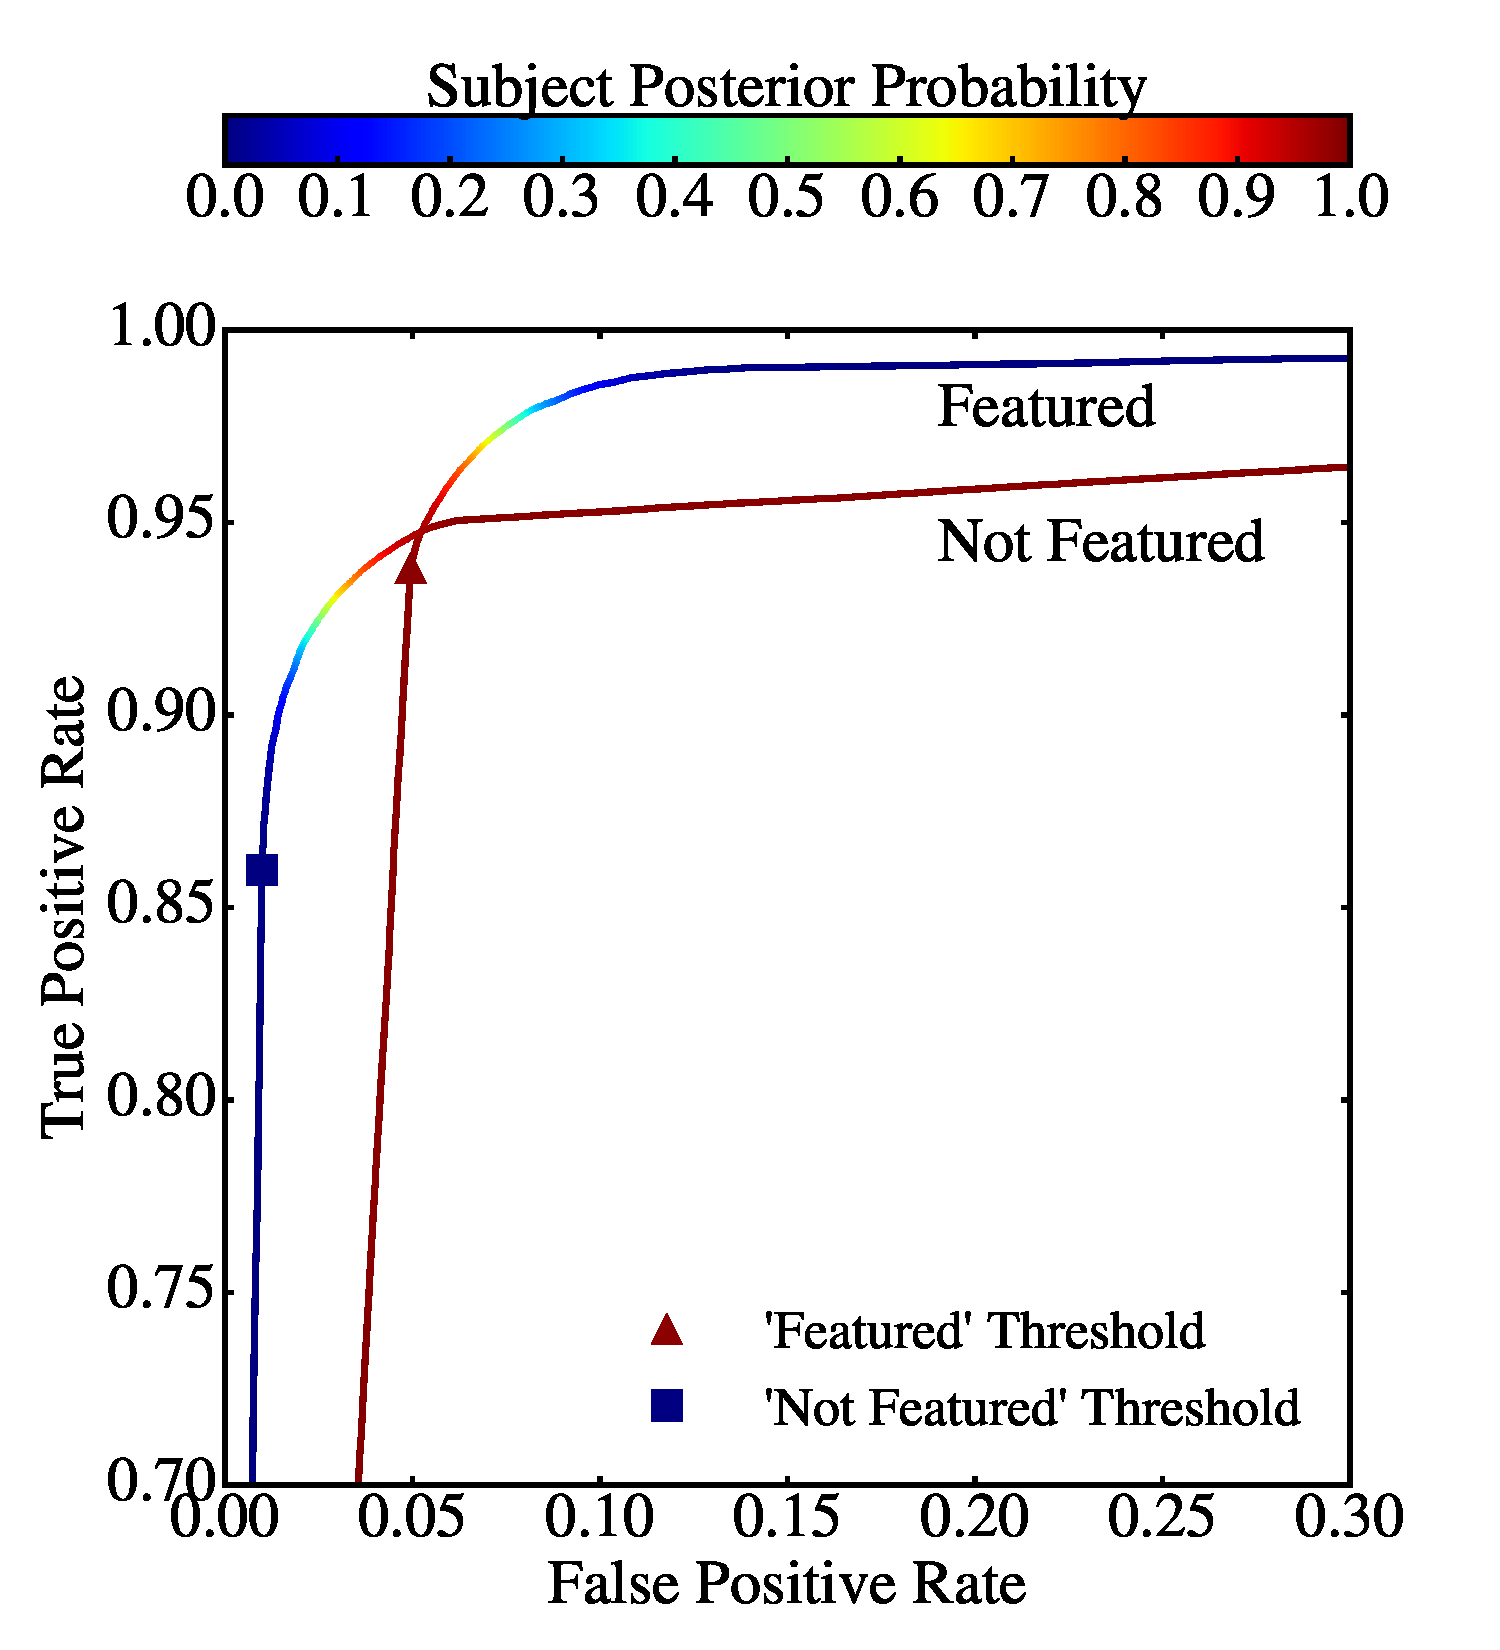
\includegraphics[width=3.25in]{figures/SWAP_ROC_curve_4paper.png}
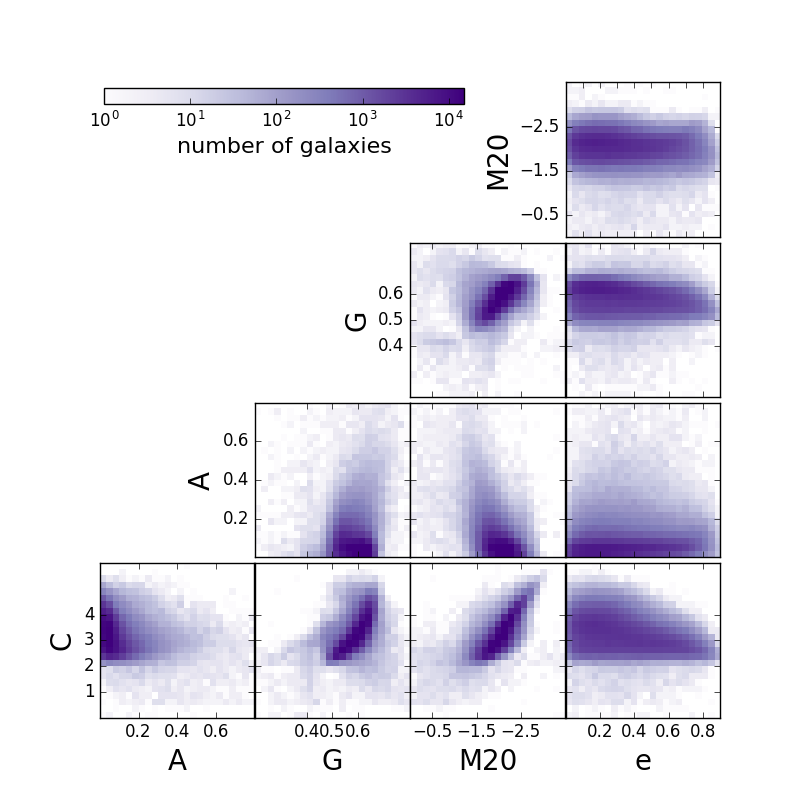
\includegraphics[width=3.55in]{figures/morph_params_entire_GZ2_sample.png}
\caption{\textit{Left.} Identifying~\feat~subjects is independent of identifying~\notfeat~subjects.  Both ROC curves use all subjects processed by SWAP where the score used to create the ROC curve is simply each subject's achieved posterior probability. The Featured curve demonstrates how well we identify~\feat~subjects with a threshold of 0.99, while the Not Featured curve demonstrates how well we identify~\notfeat~subjects with a threshold of 0.004. Typically, best performance is achieved with scores that lie closest to the upper left corner.  Our~\feat~threshold is nearly as optimumal as possible though our~\notfeat~threshold could have been slightly better. \textit{Right.} Relation between morphology diagnostics measured for more than 280K SDSS galaxies classified during the GZ2 project. \label{fig: retirement thresholds}}
\label{fig: morph thresh}
%\caption{That's a lot of parameters! \label{fig: machine classified}}
\end{figure*}



%% ----------------------------------------------------------------------------------------------------------------------------------------------
%% DISCUSSION OF CHANGING SWAP PARAMETERS
%% ----------------------------------------------------------------------------------------------------------------------------------------------
\section{Exploring SWAP's Parameter Space}
\label{sec: tweaking swap}

%% -------------------------------------------------------------------------------
%%   FIGURE:  SWAP -- adjust CONFUSION MATRIX
%% -------------------------------------------------------------------------------
\begin{figure*}[t]
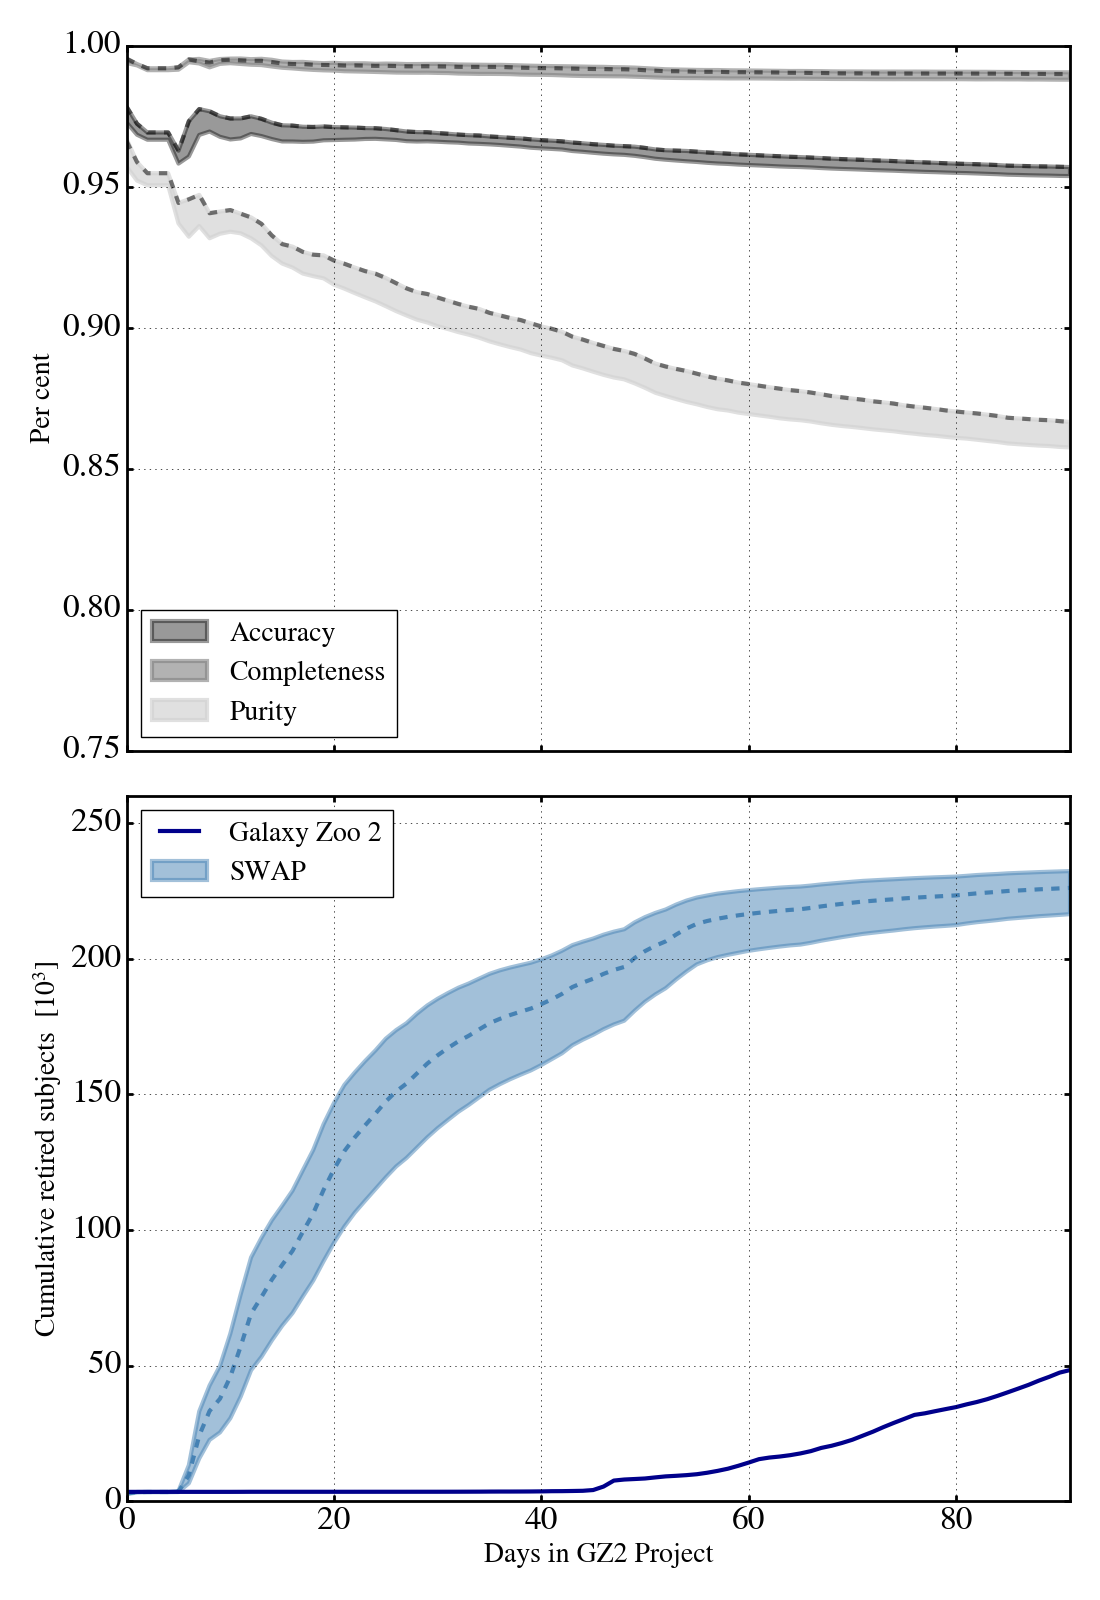
\includegraphics[width=3.35in]{figures/GZX_eval_and_retirement_PLPD_spread_4paper_v2.png}
%\caption{GZX/SWAP output as a function of GZ2 project days for a range of initial
%confusion matrix values.  \label{fig: confusionMatrixAnalysis}}
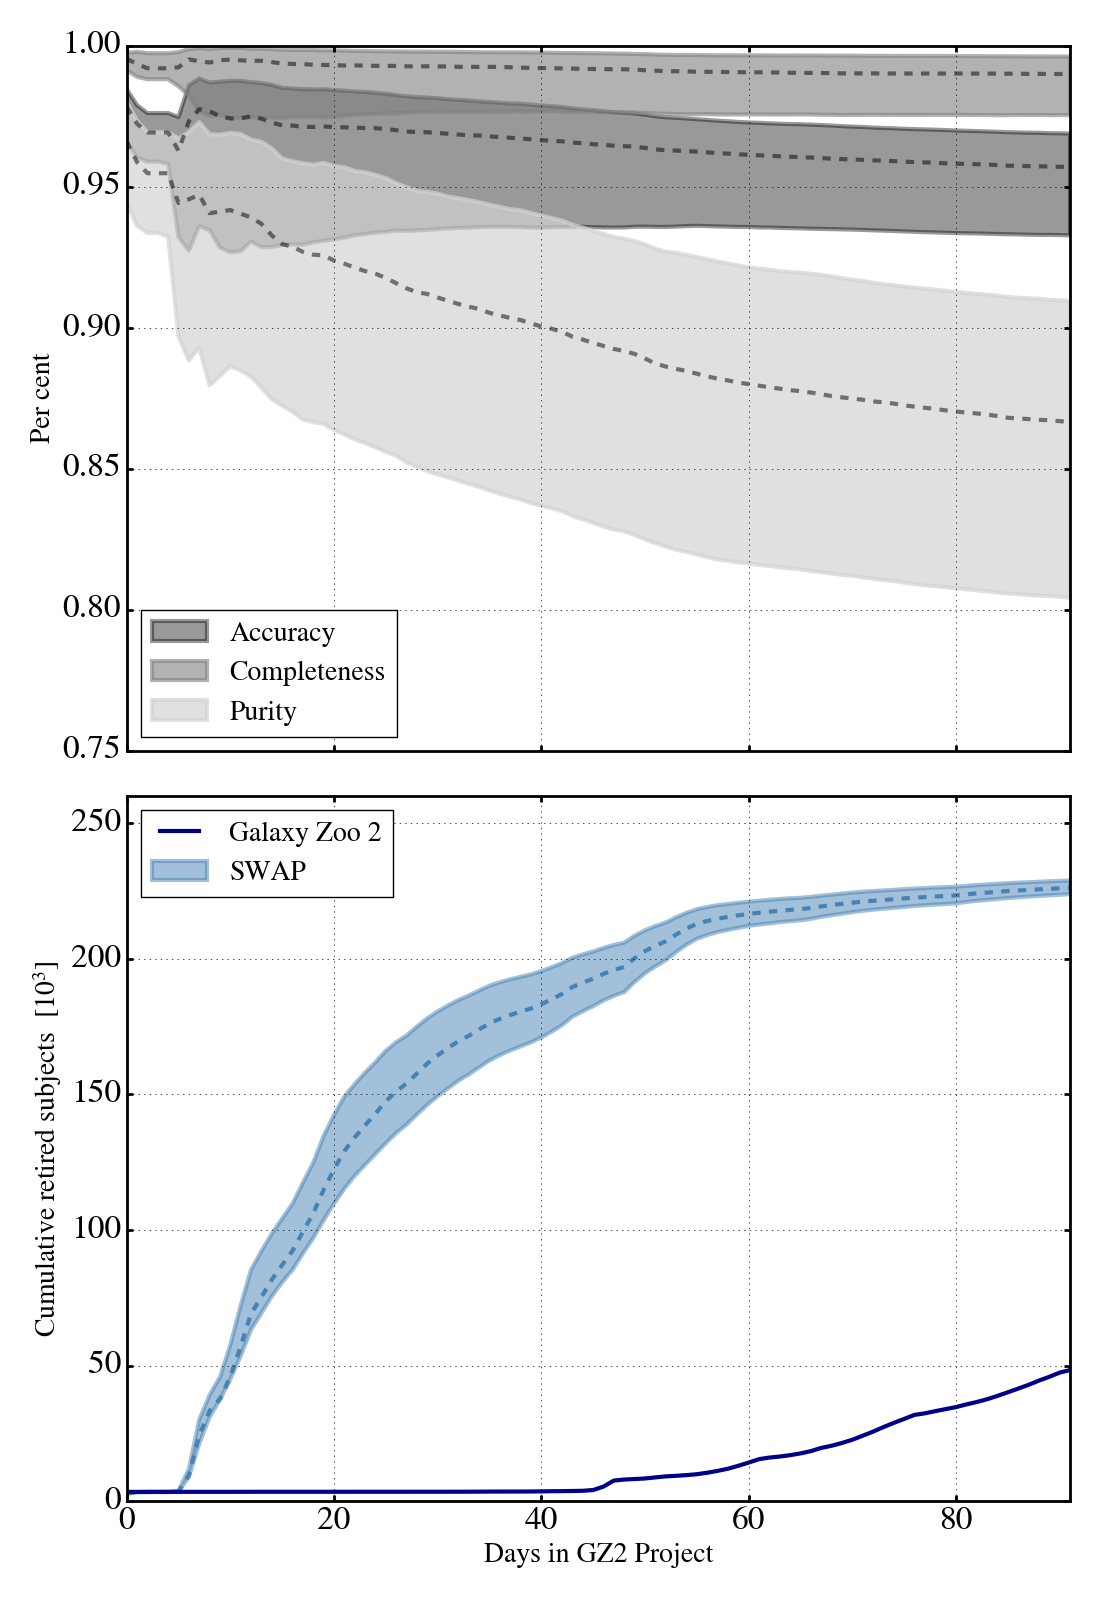
\includegraphics[width=3.35in]{figures/GZX_eval_and_retirement_prior_spread_4paper_v2.png}
\caption{SWAP output does not dramatically change for a range of SWAP parameters.  \textit{Left.} The quality (top) and retirement rate (bottom) when different values of agent confusion matrix are assigned. \textit{Right.} Same as the left panel but for various values of the subject prior probability. Changing the confusion matrix has little impact on the quality of the labels but varies the total number of subjects retired during the run. In contrast, changing the subject prior is more likelyt o affect the quality of the retirement labels rather than the total number retired. \label{fig: tweak swap}}
\end{figure*}

\textbf{Initial agent confusion matrix.} 
In our fiducial simulation each volunteer was assigned an agent with confusion matrix
 (\Pf, \Pn) = $(0.5, 0.5)$, which presumes that volunteers are no better than 
random classifiers.  We perform two simulations wherein we allow (\Pf, \Pn) = $(0.4, 0.4)$, 
slightly obtuse volunteers, and (\Pf, \Pn) = $(0.6, 0.6)$, slightly astute volunteers 
with everything else remaining constant.  
Results of these simulations compared to the fiducial run are shown in 
Figure~\ref{fig: tweak swap}. We find that we are largely insensitive to the 
initial agent confusion matrix probabilities both in terms of the overall number of retired subjects
and in the quality of their SWAP labels. 

Predictably, when (\Pf, \Pn) are low, we retire fewer subjects in the same time frame and 
more subjects when (\Pf, \Pn) are high. This is easy to understand since it takes 
longer for volunteers to become strong, astute classifiers when they are initially 
given values denoting them as obtuse. Even with this handicap, most volunteers 
become astute classifiers by the end of the simulation. Overall,  we retire 
$\sim225$K  $\pm 3.5\%$ subjects as shown by the light blue spread in the bottom
panel of Figure~\ref{fig: tweak swap} where the dashed blue line
denotes the fiducial run. 

The top panel depicts the same quality metrics computed before where the dashed 
lines again denote the fiducial run.  The spread is within a couple per cent for any
metric. Overall we maintain accuracy around $95\%$, as well as completeness of $99\%$
while maintaining purity around $84\%$. This spread can be due to three different
effects: 1) classifying a different subset of subjects, 2) retiring subjects in a different
order, and 3) subjects acquiring a different SWAP label in different simulations. 

We find that SWAP is exceptionally consistent. Of all the subjects retired in
these runs, we find that over 99\% of them are the same subjects between simulations.
Of those consistent between runs, we find that SWAP gives the same label for 
more than 99\% of the subjects. What changes between runs is the order in 
which subjects are classified. In the low (\Pf, \Pn) run, subjects take longer to classify 
compared to the fiducial run (i.e., they retire on a later date in GZ2 project time). 
Subjects in the high (\Pf, \Pn) run retire earlier in GZ2 project time. This can cause
a variation in accuracy, completeness or purity because these values are 
calculated on a day to day basis; if we're working with a slightly different make-up
of subjects on a given day, we can expect to compute different values for these metrics.
These effects each contribute less than one per cent variation and thus we see a 
high level of consistency between these simulations. 



%% -------------------------------------------------------------------------------
%%   FIGURE:  SWAP -- vary SUBJECT PRIOR
%% -------------------------------------------------------------------------------
\begin{figure}[t!]

\end{figure}


\textbf{Subject prior probability,~\p.}
The prior probability assigned to each subject is an educated guess of 
the frequency of that characteristic in the scope of the data at hand. 
For galaxy morphologies, this number should be an estimate of the probability
of observing a desired feature (bar, disk, ring, etc.). In our case, 
we desire to simply find galaxies that are~\feat, however, this is dependent 
on mass, redshift, physical size, etc. The original GZ2 sample was selected
primarily on magnitude and redshift.  As there was no cut on the galaxy size
(with the exception that each galaxy be larger than the SDSS PSF), the sample
includes a large range of galaxy masses and sizes. Thus, designating a single 
prior is not clear-cut. We thus explore how various~\p~affect the SWAP outcome.

We run several simulations where~\p~is allowed to take values 0.2, 0.35, and 0.8 
and compare these to the fiducial run where~\p~= 0.5, everything else remaining constant.
The results are shown in Figure~\ref{fig: priorAnalysis}, where again we find that 
SWAP is consistent in terms of the total number of subjects retired 
during the simulation which varies by only 1\%. 
However, as can be seen in the top panel, the variation in our quality metrics is 
more pronounced and deserves some discussion. 

Firstly, though we are retiring nearly the same number of subjects over the course
of each simulation, they are less consistent than our previous simulations. That is, 
only 95\% of the subjects are common to all runs. Secondly, of those that are 
common, only 94\% receive the same label from SWAP. Changing the prior is more
likely to produce a different label for a given subject than changing the initial 
agent confusion matrix. Finally, there is also a larger spread in the day on which 
a subject is retired when compared to the fiducial run, being nearly equally likely to 
retire `late' or `early' regardless of~\p. These trends all contribute to a broader 
spread in accuracy, completeness, and purity as a function of project time.
We stress, however, that though more substantial than the previous comparison, 
these variations are all within $\pm5\%$. 

We can get a handle on these variations more intuitively by considering the following.
Recall that our retirement thresholds,~\tf~and~\tn, have not changed in these simulations. 
Thus when~\p~is small, the subject probability is already closer to~\tn, and more 
subjects are classified as~\notfeat~compared to the fiducial run.
Similarly, when~\p~is large, some of these same subjects can instead be classified
as~\feat~because the prior probability is already closer to~\tf. Obviously, both 
outcomes cannot be correct and we find that the simulation with~\p~= 0.8 performs
the worst of any run which is a direct reflection of the fact that this prior is not 
suitable for this question nor for this dataset. For the mass, size, and redshift range
of subjects in GZ2, we would not expect that 80\% of them are~\feat. Indeed, 
the best performance is achieved when~\p = 0.35.  This reflects the actual 
distribution of~\feat~subjects in the GZ2 sample as well as being similar to the 
expected proportion of~\feat~galaxies in the local universe, depending on your
definition.
Thus, the take-away here is to choose your prior wisely since a value far from the correct
value can have a significant impact on the quality of your classifications.
 
%% ---------------------------------------------------------------------


\textbf{Retirement thresholds.}
Retirement thresholds are directly related to the time that a subject will spend
in SWAP before retiring.  If we lower~\tf~(and/or raise~\tn), more subjects will be retired
compared to the fiducial run as each subject will have a smaller swath of probability space
in which to bounce back and forth before crossing one of these thresholds.
On the other hand, if we raise~\tf~(and/or lower~\tn), it will take longer for subjects
to cross one of these thresholds. Additionally, this will also increase the likelihood of
some subjects never crossing either threshold as there are always some 
which are nudged back and forth indefinitely through probability space.


What thresholds should one choose? To answer this question, we consider
Figure~\ref{fig: retirement thresholds} which depicts the receiver operating 
characteristic (ROC) curve for our fiducial simulation. The solid line shows the 
curve when considering the~\feat~threshold  while the dotted line
corresponds to~\notfeat. The square and triangle represent our thresholds, 
(\tf,~\tn) = (0.99, 0.004), on that curve at the end of the simulation.  We see that 
~\tf~is nearly optimal but~\tn~could be improved upon. 


Throughout this discussion we have computed quality metrics under the assumption
that the `true' labels provided by GZ2 are accurate. 
This is unlikely to be the case for every subject as~\cite{Willett2013} explicitly caution against using 
the majority volunteer vote fraction as label since some of these are highly uncertain. 
We now turn to a brief discussion of those subjects where SWAP and GZ2 do not agree. 




%% The reference list follows the main body and any appendices.
%% Use LaTeX's thebibliography environment to mark up your reference list.
%% Note \begin{thebibliography} is followed by an empty set of
%% curly braces.  If you forget this, LaTeX will generate the error
%% "Perhaps a missing \item?".
%%
%% thebibliography produces citations in the text using \bibitem-\cite
%% cross-referencing. Each reference is preceded by a
%% \bibitem command that defines in curly braces the KEY that corresponds
%% to the KEY in the \cite commands (see the first section above).
%% Make sure that you provide a unique KEY for every \bibitem or else the
%% paper will not LaTeX. The square brackets should contain
%% the citation text that LaTeX will insert in
%% place of the \cite commands.

%% We have used macros to produce journal name abbreviations.
%% \aastex provides a number of these for the more frequently-cited journals.
%% See the Author Guide for a list of them.

%% Note that the style of the \bibitem labels (in []) is slightly
%% different from previous examples.  The natbib system solves a host
%% of citation expression problems, but it is necessary to clearly
%% delimit the year from the author name used in the citation.
%% See the natbib documentation for more details and options.


\bibliographystyle{apj}
\bibliography{apj-jour,human-machine}

%% This command is needed to show the entire author+affilation list when
%% the collaboration and author truncation commands are used.  It has to
%% go at the end of the manuscript.
%\allauthors

%% Include this line if you are using the \added, \replaced, \deleted
%% commands to see a summary list of all changes at the end of the article.
\listofchanges

\end{document}

%% End of file `sample.tex'.